\documentclass[11pt,a4paper]{article}
\usepackage[a4paper,margin=2.3cm]{geometry}
\usepackage{amsmath,amssymb,mathtools,amsthm}
\usepackage{fontspec}
\usepackage{polyglossia}
\setmainlanguage{russian}
\setotherlanguage{english}
\setmainfont{Liberation Serif}
\setsansfont{Liberation Sans}
\setmonofont{Liberation Mono}
\newfontfamily\cyrillicfont[Ligatures=TeX]{Liberation Serif}
\newfontfamily\cyrillicfontsf[Ligatures=TeX]{Liberation Sans}
\newfontfamily\cyrillicfonttt{Liberation Mono}
\usepackage{booktabs}
\usepackage{array}
\usepackage{enumitem}
\usepackage{graphicx}
\usepackage{float}
\usepackage{listings}
\usepackage{xcolor}
\usepackage[hidelinks]{hyperref}

\setlength{\parindent}{0pt}
\setlength{\parskip}{0.55em}
\emergencystretch=3em
\setlist{itemsep=0.25em,topsep=0.3em}
\setcounter{tocdepth}{2}
\lstset{basicstyle=\ttfamily\footnotesize,columns=fullflexible,keepspaces=true,
  frame=single,rulecolor=\color{black!25},breaklines=true,
  commentstyle=\color{black!55},showstringspaces=false}

\newcommand{\G}{\mathcal{G}_k}
\newcommand{\norm}[1]{\lVert #1\rVert_2}
\newcommand{\E}{\mathbb{E}}
\DeclareMathOperator*{\argmin}{arg\,min}
\DeclareMathOperator{\diag}{diag}
\DeclareMathOperator{\Var}{Var}
\DeclareMathOperator{\sigm}{sigm}
\makeatletter\newcommand{\tabinput}[1]{\@@input #1 }\makeatother
\renewcommand{\figurename}{Рис.}


\title{SGD против робастного SGD при неопределённости градиента\\[0.3em]
\large Отчёт по домашнему мини-проекту}
\author{Егор Чулков, Владислав Дворников, Дарья Демешко\\[0.2em]\small Optimisation methods for artificial intelligence}
\date{17 ноября 2026 г.}

\begin{document}
\maketitle

\begin{abstract}
\noindent Робастный SGD (R-SGD) выбирает каждый шаг против худшего градиента из эллипсоида $\G$,
построенного по наблюдениям мини-батча. В отчёте выводится робастный шаг, реализуется точный
решатель стоимостью $O(p)$, и SGD сравнивается с R-SGD на логистической регрессии и двухслойной
$\tanh$-сети при добавленном шуме градиента.

\emph{Теория.}
\begin{itemize}
\item Шаг единствен и никогда не длиннее шага SGD.
\item Он равен нулю тогда и только тогда, когда $g_k^TS_k^{-1}g_k\le\rho^2$; из этого не следует
$\nabla f(\theta_k)=0$.
\item В изотропном случае он выполняет мягкое пороговое отсечение нормы градиента.
\item Если истинный градиент лежит в $\G$ и $\alpha_k<2/L$, он уменьшает $f$ не менее чем на
$(\alpha_k^{-1}-L/2)\|d_k\|^2$.
\end{itemize}

\emph{Реализация.} Для диагональной $S_k$ шаг сводится к одному скалярному уравнению, для которого
доказана монотонная сходимость метода Ньютона: около 4 итераций, невязка $\le10^{-14}$.

\emph{Эксперименты.} Использован честный протокол: равные бюджеты, настройка по валидации, 10
парных сидов и контроль — SGD с той же длиной шага.
\begin{itemize}
\item \emph{Логистическая регрессия.} Оба метода достигают байесовской точности. R-SGD даёт малые,
но устойчивые выигрыши по потерям при малом шуме благодаря адаптивному сжатию, но не по точности.
\item \emph{Сеть.} R-SGD достигает в $5.8$ раза меньших потерь на обучении без шума, но SGD с той же
средней длиной шага не хуже.
\item \emph{Шум.} С настройками, зафиксированными на уровне настройки, R-SGD хуже SGD при сильном
шуме.
\end{itemize}

\emph{Объяснение.} При доминирующем изотропном шуме робастный шаг сводится к SGD с длиной шага,
умноженной на $1-\rho/\sqrt p$, а правило нулевого шага срабатывает далеко от любого минимума.
Меньшие потери при малом шуме не означали более высокой точности.
\end{abstract}

\section*{Участники и вклад}
\begin{center}
\begin{tabular}{@{}p{0.3\linewidth}p{0.62\linewidth}@{}}
\toprule
Участник & Вклад \\
\midrule
Егор Чулков & [вклад] \\
Владислав Дворников & [вклад] \\
Дарья Демешко & [вклад] \\
\bottomrule
\end{tabular}
\end{center}

\newpage
\tableofcontents
\newpage


\section{Вывод и интерпретация}\label{sec:derivation}

Всюду $\alpha_k>0$, $\rho\ge0$ и $S_k\succ0$. Внутри одного шага индекс $k$ опускается:
$g=g_k$, $S=S_k$, $\alpha=\alpha_k$. Поскольку $S\succ0$, у неё есть спектральное разложение
$S=Q\Lambda Q^T$ с ортогональной $Q$ и $\Lambda=\diag(\lambda_i)$, $\lambda_i>0$. Поэтому матрицы
$S^{1/2}=Q\Lambda^{1/2}Q^T$ и $S^{-1/2}=Q\Lambda^{-1/2}Q^T$ существуют, симметричны и
положительно определены, причём $S^{-1/2}S^{-1/2}=S^{-1}$ и $\sqrt{x^TSx}=\norm{S^{1/2}x}$.

\subsection{(a) Робастная линейная задача}

Рассмотрим $\min_{x\in X}\max_{c\in\mathcal C}c^Tx$, где
$\mathcal C=\{\mu+S^{1/2}u:\norm u\le\rho\}$.

\textbf{Внутренний максимум.} При фиксированном $x$, пользуясь симметричностью $S^{1/2}$,
\begin{equation*}
\max_{\norm u\le\rho}(\mu+S^{1/2}u)^Tx=\mu^Tx+\max_{\norm u\le\rho}u^T\big(S^{1/2}x\big)
=\mu^Tx+\rho\,\norm{S^{1/2}x}=\mu^Tx+\rho\sqrt{x^TSx}.
\end{equation*}
Среднее равенство — это неравенство Коши — Буняковского $u^Tv\le\norm u\norm v\le\rho\norm v$
при $v=S^{1/2}x$; оно обращается в равенство при $u=\rho v/\norm v$.

\textbf{Точка максимума при $x\ne0$.} Матрица $S^{1/2}$ обратима, поэтому $v=S^{1/2}x\ne0$ и
\begin{equation*}
u^\star=\rho\,\frac{S^{1/2}x}{\norm{S^{1/2}x}},\qquad
c^\star=\mu+S^{1/2}u^\star=\mu+\rho\,\frac{Sx}{\sqrt{x^TSx}} .
\end{equation*}
При $\rho>0$ она единственна: равенство в неравенстве Коши — Буняковского при $\norm u=\rho$
требует, чтобы $u$ было положительно кратно $v$. При $x=0$ максимумом является любое $u$, и
значение равно $0$. Значит, робастная линейная задача — это выпуклая задача
$\min_{x\in X}\mu^Tx+\rho\sqrt{x^TSx}$ (задача конического программирования второго порядка
при многогранном $X$). Противник сдвигает вектор стоимости от номинального $\mu$ в направлении
$Sx$, то есть вдоль самых неопределённых направлений, в которых движется $x$.

\textbf{Локальная модель градиента.} Вблизи $\theta_k$ имеем
$f(\theta_k+d)\approx f(\theta_k)+\nabla f(\theta_k)^Td$. Истинный градиент неизвестен; данные
говорят лишь, что он правдоподобно лежит в $\G$. Отождествив решение $x\mapsto d$, номинальную
стоимость $\mu\mapsto g_k$ и форму $S\mapsto S_k$, получаем модель убывания первого порядка в
худшем случае. Линейная модель не ограничена снизу, поэтому вместо множества $X$ шаг удерживает
локальным проксимальное слагаемое $\norm d^2/(2\alpha_k)$; это и есть задача (1).

\subsection{(b) Эквивалентная формулировка и робастный шаг}

Проксимальное слагаемое не зависит от $h$, поэтому выносится из внутреннего максимума, и пункт (a)
при $x=d$, $\mu=g$ даёт
\begin{equation*}
\varphi(d):=\max_{h\in\G}\Big\{h^Td+\frac{\norm d^2}{2\alpha}\Big\}
=g^Td+\rho\sqrt{d^TSd}+\frac{\norm d^2}{2\alpha},\qquad d_k=\argmin_d\varphi(d),
\end{equation*}
то есть формулу (2).

\textbf{При $\rho=0$ получается SGD.} Тогда $\varphi(d)=g^Td+\norm d^2/(2\alpha)$ — строго выпуклая
квадратичная функция с градиентом $g+d/\alpha$; её единственная точка минимума $d_k=-\alpha g$ —
шаг SGD.

\textbf{Существование и единственность.} $\varphi$ — сумма линейной функции, выпуклой функции
$\rho\norm{S^{1/2}d}$ (норма линейного отображения) и $1/\alpha$-сильно выпуклой квадратичной
функции $\norm d^2/(2\alpha)$. Поэтому $\varphi$ непрерывна и $1/\alpha$-сильно выпукла. Кроме
того, она коэрцитивна: $\varphi(d)\ge-\norm g\norm d+\norm d^2/(2\alpha)\to\infty$. Непрерывная
коэрцитивная функция достигает минимума, а сильная выпуклость делает точку минимума
единственной. Итак, при любых $g$, $S\succ0$, $\rho\ge0$, $\alpha>0$ робастный шаг $d_k$ существует
и единствен, хотя при $\rho>0$ функция $\varphi$ не дифференцируема в $d=0$. Точно он вычисляется в
разделе~\ref{sec:impl}.

\textbf{Робастный шаг никогда не длиннее шага SGD.} При $d_k\ne0$ условие оптимальности из
пункта (d), умноженное на $d_k^T$, даёт $g^Td_k+\rho\sqrt{d_k^TSd_k}+\norm{d_k}^2/\alpha=0$,
откуда $\norm{d_k}^2/\alpha=-g^Td_k-\rho\sqrt{d_k^TSd_k}\le\norm g\norm{d_k}$ и
$\norm{d_k}\le\alpha\norm{g_k}$.

\subsection{(c) Условие нулевого шага}

\textbf{Результат.}
\begin{equation*}
\boxed{\;d_k=0\iff g_k^TS_k^{-1}g_k\le\rho^2\iff0\in\G\;}
\end{equation*}
Из условия (3) \emph{не} следует $\nabla f(\theta_k)=0$.

\textbf{(3) $\iff0\in\G$.} $0\in\G$ означает $g+S^{1/2}u=0$ при некотором $\norm u\le\rho$.
Матрица $S^{1/2}$ обратима, поэтому единственный кандидат $u=-S^{-1/2}g$, и
$\norm u^2=g^TS^{-1/2}S^{-1/2}g=g^TS^{-1}g$. Величина $\kappa=\sqrt{g^TS^{-1}g}$ — норма
Махаланобиса вектора $g$: усреднённый градиент в единицах его собственной оценённой
неопределённости, то есть отношение сигнал/шум.

\textbf{(3) $\Rightarrow d_k=0$.} Заметим, что $\varphi(0)=0$. При $d\ne0$, вставив
$S^{-1/2}S^{1/2}=I$ и применив неравенство Коши — Буняковского,
\begin{equation*}
g^Td=(S^{-1/2}g)^T(S^{1/2}d)\ge-\kappa\sqrt{d^TSd}\ge-\rho\sqrt{d^TSd}
\quad\Longrightarrow\quad
\varphi(d)\ge\frac{\norm d^2}{2\alpha}>0=\varphi(0).
\end{equation*}
Значит, $d=0$ — единственная точка минимума. То же из (1): если $0\in\G$, противник может выбрать
$h=0$, и $\varphi(d)\ge\norm d^2/(2\alpha)>0$ при $d\ne0$.

\textbf{$d_k=0\Rightarrow$ (3).} Если $d_k=0$, то $\varphi(d)\ge0$ при всех $d$. Возьмём
$d(t)=-tS^{-1}g$, $t>0$: $\varphi(d(t))=-t\kappa^2+\rho t\kappa+t^2\norm{S^{-1}g}^2/(2\alpha)\ge0$.
Разделив на $t$ и устремив $t\to0^+$, получаем $\kappa(\rho-\kappa)\ge0$, то есть $\kappa\le\rho$
(при $\kappa=0$ — тривиально).

\textbf{То же через условие оптимальности.} Функция $d\mapsto\norm{S^{1/2}d}$ — опорная функция
эллипсоида $\{S^{1/2}u:\norm u\le1\}$, а субдифференциал опорной функции в нуле равен самому
множеству. Поэтому $\partial\varphi(0)=\{g+\rho S^{1/2}u:\norm u\le1\}=\G$, и правило Ферма
$0\in\partial\varphi(0)$ — это в точности $0\in\G$. Порог не зависит от $\alpha_k$: шаг обучения
масштабирует ненулевой шаг, но не может ни создать, ни убрать нулевой.

\textbf{Следует ли из (3), что $\nabla f(\theta_k)=0$? Нет.}
\begin{itemize}
\item В (3) входят только выборочные величины $g_k$, $S_k$ и настраиваемый параметр $\rho$;
истинный градиент в нём не участвует. Большее $\rho$, более шумный батч или меньшее $b$ (так как
$S_k\propto1/b$) делают (3) верным в любой точке.
\item Даже если $\nabla f(\theta_k)\in\G$ (предположение пункта (e)), при $\rho>0$ множество $\G$ —
полноразмерный эллипсоид, содержащий кроме нуля бесконечно много ненулевых векторов.
\item Контрпример по формуле (4): $f(\theta)=\tfrac12\theta^2$, $\theta_k=1$,
$\nabla f(\theta_k)=1$, $b=2$ наблюдения $v_{k,1}=3$, $v_{k,2}=-1$. Тогда $g_k=1$,
$\widehat s_k=\tfrac12(2^2+2^2)=4$, $\varepsilon_k=0.004$, $s_k=4.004$ и
$g_k^2/s_k=0.2498\le1=\rho^2$ при $\rho=1$. Значит, $d_k=0$, хотя $\nabla f(\theta_k)\ne0$, оценка
точна и SGD сделал бы правильный шаг. Среднее отстоит от нуля на половину стандартной ошибки, и по
двум наблюдениям нельзя отличить градиент $1$ от градиента $0$.
\end{itemize}
Правильное прочтение — статистическое: (3) означает, что нулевой градиент не исключён при радиусе
$\rho$. Импликация верна лишь при $\rho=0$ вместе с $\nabla f(\theta_k)\in\G$; обратная тоже
неверна, так как в стационарной точке шумный $g_k$ может нарушить (3). Поэтому нулевые шаги
возникают ещё до минимума — там, где градиент мал по сравнению со своим шумом (разделы~\ref{sec:checks}
и \ref{sec:critical}).

\subsection{(d) Условие оптимальности и изотропный случай}

\textbf{Ненулевой шаг.} При $d\ne0$ имеем $d^TSd>0$, поэтому $\varphi$ дифференцируема в $d$ и
$\nabla_d\sqrt{d^TSd}=Sd/\sqrt{d^TSd}$. Так как $\varphi$ выпукла, $d_k\ne0$ — точка минимума тогда
и только тогда, когда
\begin{equation*}
g_k+\rho\,\frac{S_kd_k}{\sqrt{d_k^TS_kd_k}}+\alpha_k^{-1}d_k=0 .
\end{equation*}
Эквивалентно $d_k=-\alpha_kh^\star$, где $h^\star=g_k+\rho S_kd_k/\sqrt{d_k^TS_kd_k}\in\G$ —
градиент худшего случая из пункта (a): R-SGD делает шаг SGD вдоль худшего правдоподобного
градиента.

\textbf{Изотропный случай $S_k=sI$, $g_k\ne0$.} Тогда $\sqrt{d^TSd}=\sqrt s\norm d$, и условие
принимает вид $\big(\alpha^{-1}+\rho\sqrt s/\norm d\big)d=-g$. Скобка положительна, поэтому
$d=-tg/\norm g$ с $t=\norm d>0$. Подстановка даёт $\norm g-\rho\sqrt s-t/\alpha=0$, то есть
$t=\alpha(\norm g-\rho\sqrt s)$, что допустимо лишь при $\norm g>\rho\sqrt s$. Если же
$\norm g\le\rho\sqrt s$, то есть $g^TS^{-1}g=\norm g^2/s\le\rho^2$, по пункту (c) $d_k=0$. Вместе:
\begin{equation*}
\boxed{\;d_k=-\alpha_k\Big(1-\frac{\rho\sqrt s}{\norm{g_k}}\Big)_+g_k\;}
\end{equation*}

\textbf{Случай $g_k=0$.} Тогда $\varphi(d)=\rho\sqrt s\norm d+\norm d^2/(2\alpha)>0=\varphi(0)$ при
$d\ne0$, поэтому $d_k=0$ — в согласии с (3), так как $0\le\rho^2$. Формулу выше читаем с этим
соглашением, поскольку отношение в ней при $g_k=0$ не определено.

\textbf{Влияние изотропной и анизотропной неопределённости.}
\begin{itemize}
\item \emph{Изотропная:} направление как у SGD; меняется только длина — мягким порогом по норме
градиента, $\norm{d_k}=\alpha_k(\norm{g_k}-\rho\sqrt s)_+$. Малые (шумные) градиенты сжимаются
относительно сильнее, большие проходят почти без изменений.
\item \emph{Анизотропная:} из условия $d_k=-\alpha\big(I+\alpha\rho S/\tau\big)^{-1}g$, где
$\tau=\sqrt{d_k^TSd_k}$. Направления с большой неопределённостью (большими собственными числами
$S$) гасятся сильнее, поэтому шаг ещё и поворачивается. Для диагональной $S$
$d_{k,j}=-\alpha\tau g_j/(\tau+\alpha\rho s_j)$; при $\rho\to0$ направление стремится к $-g$, а при
росте $\rho$ к порогу $\kappa$ — к $-S^{-1}g$, градиенту в единицах его неопределённости
(раздел~\ref{sec:impl}, рис.~\ref{fig:sweep}).
\end{itemize}

\subsection{(e) Условное убывание}

\textbf{Утверждение.} Если $\nabla f(\theta_k)\in\G$ и $\nabla f$ липшицев с константой $L$, то
неравенство
\begin{equation*}
f(\theta_k+d_k)\le f(\theta_k)-\big(\alpha_k^{-1}-L/2\big)\norm{d_k}^2
\end{equation*}
\emph{выполнено}.

\textbf{Доказательство.} При $d_k=0$ обе части равны $f(\theta_k)$. Пусть $d=d_k\ne0$.
\begin{enumerate}
\item Лемма о спуске (липшицев градиент):
$f(\theta_k+d)\le f(\theta_k)+\nabla f(\theta_k)^Td+\tfrac L2\norm d^2$.
\item Включение: $\nabla f(\theta_k)\in\G$, поэтому
$\nabla f(\theta_k)^Td\le\max_{h\in\G}h^Td=g^Td+\rho\sqrt{d^TSd}$ по пункту (a).
\item Оптимальность: умножив условие пункта (d) на $d^T$, получаем
$g^Td+\rho\sqrt{d^TSd}=-\norm d^2/\alpha$.
\end{enumerate}
Вместе: $f(\theta_k+d)\le f(\theta_k)-\norm d^2/\alpha+\tfrac L2\norm d^2$. \hfill$\blacksquare$

\textbf{Достаточное условие на шаг.} При $\alpha_k<2/L$ множитель $\alpha_k^{-1}-L/2>0$, и
$f(\theta_{k+1})<f(\theta_k)$ при любом $d_k\ne0$; например, $\alpha_k\le1/L$ гарантирует убывание не
менее чем на $\tfrac L2\norm{d_k}^2$.

\textbf{Роль включения.} Шаг~2 доказательства — единственное место, где участвует истинный
градиент. Без $\nabla f(\theta_k)\in\G$ слагаемое $\nabla f(\theta_k)^Td$ может быть положительным, и
убывание не гарантировано: $d_k$ — направление убывания для каждого градиента из $\G$, но не
обязательно для градиента вне его. Включение — случайное событие, которое по данным проверить нельзя.
В гауссовском приближении при $S_k$, равной истинной ковариации $g_k$, его вероятность
$P(\chi^2_p\le\rho^2)$: большее $\rho$ делает гарантию вероятнее, но укорачивает шаги и порождает
больше нулевых шагов (раздел~\ref{sec:critical}). При оценённой $S_k$ и малом $b$ вероятность ниже.
На многих итерациях гарантия требует включения на каждом шаге, так что это утверждение об одном
шаге, а не теорема о сходимости. При $\rho=0$ включение означает $g_k=\nabla f(\theta_k)$ точно, и
результат сводится к классическому убыванию градиентного спуска с точными градиентами.


\section{Реализация и численные проверки}\label{sec:impl}

В этом разделе строится матрица неопределённости (4), выводится точный решатель для (2),
реализуются SGD и R-SGD с оракулами градиента для обеих обучаемых моделей, и всё проверяется
численно на зашумлённой квадратичной функции из раздела Illustration. Все числа получены скриптом
\texttt{checks\_section2.py} и сохранены в \texttt{results\_section2.json}.


На итерации $k$ имеется $b\ge2$ наблюдений $v_{k,i}\in\mathbb R^p$ и
\begin{gather*}
g_k=\frac1b\sum_{i=1}^b v_{k,i},\qquad
\G=\{g_k+S_k^{1/2}u:\norm{u}\le\rho\},\\
d_k=\argmin_d\;\varphi_k(d),\qquad
\varphi_k(d)=g_k^Td+\rho\sqrt{d^TS_kd}+\frac{\norm{d}^2}{2\alpha_k}.
\end{gather*}
SGD делает шаг $\theta_{k+1}=\theta_k-\alpha_kg_k$, R-SGD — шаг
$\theta_{k+1}=\theta_k+d_k$. Внутри одного шага индекс $k$ опускается: $g$,
$S=\diag(s_1,\dots,s_p)$, $\alpha$. Норма Махаланобиса вектора $g$ и порог нулевого
шага:
\begin{equation*}
\kappa^2=g^TS^{-1}g=\sum_{j=1}^p\frac{g_j^2}{s_j},\qquad \rho_c=\kappa .
\end{equation*}

\textbf{Тестовая задача (Illustration).}
$f(\theta)=\tfrac12(\theta_1^2+4\theta_2^2)$, $\nabla f(\theta)=(\theta_1,4\theta_2)^T$,
гессиан $\diag(1,4)$, поэтому $L=4$ и $\mu=1$; $\theta_0=(2,2)^T$, $f(\theta_0)=10$,
$f^\star=0$. Наблюдения $v_{k,i}=\nabla f(\theta_k)+\sigma Az_{k,i}$, $A=\diag(2,\tfrac12)$,
$z_{k,i}\sim\mathcal N(0,I_2)$, так что ковариация одного наблюдения
\begin{equation*}
\Sigma=\sigma^2AA^T=\sigma^2\diag\big(4,\tfrac14\big).
\end{equation*}
Шум велик вдоль $\theta_1$, где кривизна мала, и мал вдоль $\theta_2$, где кривизна
велика: отношение сигнал/шум в двух направлениях сильно различается. Поскольку
$\Sigma$ диагональна, диагональная оценка (4) здесь ничего не теряет; в обучаемых
моделях она пренебрегает корреляциями между параметрами.

\subsection{Матрица неопределённости $S_k$, формула (4)}\label{sec:S}

\begin{equation*}
\widehat s_{k,j}=\frac1{b(b-1)}\sum_{i=1}^b(v_{k,i,j}-g_{k,j})^2,\qquad
s_{k,j}=\widehat s_{k,j}+\varepsilon_k,\qquad
\varepsilon_k=10^{-3}\max\Big\{\frac1p\sum_j\widehat s_{k,j},\,10^{-8}\Big\}.
\end{equation*}

\subsubsection*{Что оценивает $\widehat s_{k,j}$}

Пусть при фиксированном $\theta_k$ наблюдения независимы и одинаково распределены со
средним $m$ и ковариацией $\Sigma$. Для обучаемых моделей именно это обеспечивает
выбор примеров \emph{с возвращением} (в разделе~\ref{sec:batch} показано, что происходит без него).
Тогда $\Var(g_{k,j})=\Sigma_{jj}/b$. Из тождества
\begin{equation*}
\sum_{i=1}^b(v_{i,j}-g_j)^2=\sum_{i=1}^b(v_{i,j}-m_j)^2-b\,(g_j-m_j)^2
\end{equation*}
после взятия математического ожидания получаем
$\E\sum_i(v_{i,j}-g_j)^2=b\Sigma_{jj}-\Sigma_{jj}=(b-1)\Sigma_{jj}$. Делим на $b(b-1)$:
\begin{equation*}
\boxed{\;\E\,\widehat s_{k,j}=\frac{\Sigma_{jj}}b=\Var(g_{k,j})\;}
\end{equation*}
Таким образом, $S_k$ — это (диагональ) ковариации \emph{среднего по батчу}, а не
одного наблюдения. Это правильный объект: множество $\G$ описывает неопределённость
именно $g_k$.

\subsubsection*{Положительная определённость и роль $\varepsilon_k$}

Каждое $s_{k,j}\ge\varepsilon_k\ge10^{-11}>0$, поэтому всегда $S_k\succ0$. Добавка
нужна в двух ситуациях: координата, по которой все наблюдения совпадают (например,
насыщенный нейрон $\tanh$ или смещение модели с одинаковыми градиентами примеров), и
квадратичная задача без шума ($\sigma=0$), где все $v_{k,i}$ совпадают и
$\widehat s_k=0$. Относительная часть $10^{-3}\cdot\text{mean}(\widehat s)$ делает
добавку инвариантной к масштабу: она ограничивает отношение $\max_js_j/\min_js_j$
величиной порядка $10^3p$. Абсолютная часть $10^{-11}$ работает, только когда все
$\widehat s_{k,j}$ равны нулю. Тогда $S_k=\varepsilon_kI$, и по изотропной формуле из 1(d)
шаг R-SGD равен $d_k=-\alpha_k(1-\rho\sqrt{\varepsilon_k}/\norm{g_k})_+g_k$. Это SGD с
относительным изменением $\rho\sqrt{\varepsilon_k}/\norm{g_k}$, кроме крошечной
области $\norm{g_k}\le\rho\sqrt{\varepsilon_k}\approx3.2\cdot10^{-6}\rho$; это
проверено численно в разделе~\ref{sec:checks}.

\subsection{Решатель робастной подзадачи (2)}\label{sec:solver}

\subsubsection*{Тривиальные случаи}
\begin{itemize}
\item $\rho=0$: $\varphi(d)=g^Td+\norm d^2/(2\alpha)$, откуда $d=-\alpha g$ (SGD),
пункт 1(b).
\item $\kappa^2=g^TS^{-1}g\le\rho^2$: $d=0$, пункт 1(c). Эта проверка точна и стоит
$O(p)$. Шаг считается \emph{нулевым} только тогда, когда сработала эта проверка, а не
по сравнению $\norm d$ с допуском. Случай $g=0$ сюда входит ($\kappa=0\le\rho$).
\end{itemize}

\subsubsection*{Сведение к одному скалярному уравнению}

Пусть $\rho>0$ и $\kappa>\rho$. По пункту 1(c) точка минимума $d\neq0$, поэтому
$\varphi$ в ней дифференцируема и выполнено условие из 1(d):
\begin{equation*}
g+\rho\frac{Sd}{\sqrt{d^TSd}}+\frac d\alpha=0 .
\end{equation*}
Введём неизвестный скаляр $\tau=\sqrt{d^TSd}>0$. Так как $S$ диагональна, векторное
уравнение распадается на $p$ скалярных: $g_j+\rho s_jd_j/\tau+d_j/\alpha=0$, то есть
$d_j\big(\tfrac1\alpha+\tfrac{\rho s_j}{\tau}\big)=-g_j$. Умножая на $\alpha\tau$,
получаем
\begin{equation*}
\boxed{\;d_j(\tau)=-\alpha\,\frac{\tau}{\tau+\alpha\rho s_j}\,g_j,\qquad j=1,\dots,p\;}
\end{equation*}
При любом $\tau>0$ вектор $d(\tau)$ удовлетворяет условию оптимальности, \emph{в
котором $\sqrt{d^TSd}$ заменено на $\tau$}. Решением он является тогда и только тогда,
когда $\tau$ согласовано со своим определением: $\tau^2=\sum_js_jd_j(\tau)^2$.
Подставляя $d_j(\tau)$ и деля на $\tau^2>0$, получаем \emph{секулярное уравнение}
\begin{equation*}
q(\tau):=\sum_{j=1}^p\frac{a_j}{(\tau+c_j)^2}=1,\qquad
a_j=\alpha^2s_jg_j^2\ge0,\quad c_j=\alpha\rho s_j>0 .
\end{equation*}
(Название пришло из подзадачи доверительной области, где возникает уравнение того же
вида; см.\ Moré, Sorensen, 1983; Nocedal, Wright, 2006, §4.3.)

\subsubsection*{Существование и единственность корня $\Longleftrightarrow$ (3) нарушено}

Так как $g\ne0$, хотя бы одно $a_j>0$, и
\begin{equation*}
q'(\tau)=-2\sum_j\frac{a_j}{(\tau+c_j)^3}<0\quad(\tau\ge0),\qquad
q(0)=\sum_j\frac{\alpha^2s_jg_j^2}{\alpha^2\rho^2s_j^2}=\frac{\kappa^2}{\rho^2},\qquad
\lim_{\tau\to\infty}q(\tau)=0 .
\end{equation*}
Функция $q$ непрерывна и строго убывает, поэтому уравнение $q(\tau)=1$ имеет корень на
$(0,\infty)$ тогда и только тогда, когда $q(0)>1$, то есть $\kappa>\rho$, и этот корень
$\tau^\star$ единственен. При $\kappa\le\rho$ корня нет, то есть ни одна ненулевая
точка не удовлетворяет условию оптимальности, и минимум (он существует, поскольку
$\varphi$ сильно выпукла) обязан достигаться в $d=0$. Тем самым правило нулевого шага
1(c) содержится в решателе как случай отсутствия корня его собственного уравнения.
Поскольку задача (2) $1/\alpha$-сильно выпукла, стационарная точка $d(\tau^\star)$ —
её единственный глобальный минимум.

\textbf{Отрезок локализации.} Так как $c_j>0$, имеем
$q(\tau)\le\sum_ja_j/\tau^2=\alpha^2g^TSg/\tau^2$. Значит, $q(\tau_{\rm hi})\le1$ при
$\tau_{\rm hi}=\alpha\sqrt{g^TSg}$, и $\tau^\star\in(0,\tau_{\rm hi}]$.

\subsubsection*{Метод Ньютона для $\psi(\tau)=q(\tau)^{-1/2}-1$}

Вместо $q(\tau)-1$ (выпуклой функции, ведущей себя как $1/\tau^2$) решается уравнение
$\psi(\tau)=q(\tau)^{-1/2}-1=0$. Функция $\psi$ возрастает ($q$ убывает) и обладает
следующим ключевым свойством.

\textbf{Лемма (вогнутость).} $\psi$ вогнута на $[0,\infty)$; она аффинна тогда и
только тогда, когда все $s_j$ с $g_j\ne0$ равны между собой.

\emph{Доказательство.} Обозначим $x_j=1/(\tau+c_j)$ и $A_m=\sum_ja_jx_j^m$. Тогда
$q=A_2$, $q'=-2A_3$, $q''=6A_4$. Для $F=q^{-1/2}$
\begin{equation*}
F'=-\tfrac12q^{-3/2}q',\qquad
F''=q^{-5/2}\Big(\tfrac34q'^2-\tfrac12q\,q''\Big)=3\,q^{-5/2}\big(A_3^2-A_2A_4\big).
\end{equation*}
По неравенству Коши — Буняковского для векторов $(\sqrt{a_j}\,x_j)_j$ и
$(\sqrt{a_j}\,x_j^2)_j$ имеем $A_3^2\le A_2A_4$, поэтому $F''\le0$. Равенство
достигается тогда и только тогда, когда эти векторы пропорциональны, то есть $x_j$
одинаковы для всех $j$ с $a_j>0$, то есть все такие $c_j=\alpha\rho s_j$ совпадают.
\hfill$\blacksquare$

\textbf{Монотонная сходимость из $\tau_0=0$.} Имеем $\psi(0)=\rho/\kappa-1<0$.
Итерация Ньютона: $\tau_{n+1}=\tau_n-\psi(\tau_n)/\psi'(\tau_n)$, где $\psi'>0$. В силу
вогнутости касательная лежит не ниже графика:
$\psi(\tau)\le\psi(\tau_n)+\psi'(\tau_n)(\tau-\tau_n)$. В точке $\tau=\tau_{n+1}$
правая часть равна нулю, поэтому $\psi(\tau_{n+1})\le0$, то есть
$\tau_{n+1}\le\tau^\star$. Кроме того,
$\tau_{n+1}-\tau_n=-\psi(\tau_n)/\psi'(\tau_n)\ge0$. Итерации монотонно возрастают и
остаются не выше $\tau^\star$; их предел $\bar\tau$ удовлетворяет $\psi(\bar\tau)=0$
(непрерывность и $\psi'\ge\psi'(\tau^\star)>0$ на $[0,\tau^\star]$ в силу вогнутости),
поэтому $\bar\tau=\tau^\star$. Так как $\psi$ гладкая и $\psi'(\tau^\star)>0$,
сходимость локально квадратичная. В изотропном случае $\psi$ аффинна, и первый же шаг
Ньютона попадает точно в $\tau^\star$.

Почему $q^{-1/2}$, а не $q-1$: в изотропном случае $q^{-1/2}=(\tau+c)/\sqrt{\sum a_j}$ —
прямая, а при анизотропии функция остаётся близкой к прямой, поэтому Ньютону нужно
очень мало шагов. Для $q-1$ метод Ньютона из $\tau_0=0$ тоже монотонен (выпуклая
убывающая функция), но сходится гораздо медленнее.

\textbf{Страховка.} Итерация хранит отрезок $[\tau_{\rm lo},\tau_{\rm hi}]$ и заменяет
любую итерацию Ньютона, вышедшую за него, шагом бисекции. По доказанному выше в точной
арифметике этого не происходит; на 20\,000 тестовых задачах страховка не сработала ни
разу.

\subsubsection*{Критерий остановки и апостериорная проверка}

Итерации прекращаются, когда $|\psi(\tau_n)|\le10^{-14}$, или когда изменение
$|\tau_{n+1}-\tau_n|\le10^{-15}\tau_{n+1}$, или после 100 итераций (наблюдаемый
максимум — 9). Возвращается $d=d(\tau_n)$.

Что контролирует критерий: $d(\tau)$ удовлетворяет условию оптимальности точно, с
$\tau$ вместо $\sqrt{d^TSd}$, и
$\sqrt{d(\tau)^TSd(\tau)}=\tau\sqrt{q(\tau)}=\tau/(1+\psi(\tau))$. Значит, единственная
ошибка — относительное расхождение $|\psi|$ между $\tau$ и $\sqrt{d^TSd}$. После решения
код дополнительно вычисляет невязку условия 1(d)
\begin{equation*}
r(d)=\frac{\norm{g+\rho Sd/\sqrt{d^TSd}+d/\alpha}}{\norm g}
\end{equation*}
и сохраняет её (раздел~\ref{sec:checks}).

\subsubsection*{Вычислительная стоимость}

\begin{itemize}
\item Предвычисление $a_j$, $c_j$, $\kappa^2$ стоит $O(p)$; каждая итерация Ньютона
вычисляет две суммы, $O(p)$; память $O(p)$. Итого $O(p\cdot n_{\rm it})$, где
наблюдалось $n_{\rm it}\le9$.
\item Построение $g_k$ и $S_k$ по $V\in\mathbb R^{b\times p}$ стоит $O(bp)$, а
вычисление $b$ градиентов отдельных примеров — $O(b\cdot\text{(один backprop)})$, что
уже не меньше $O(bp)$. Асимптотически решатель дешевле данных, которые он получает,
примерно в $b/n_{\rm it}$ раз.
\item \textbf{Измеренное время (Python/NumPy, одно ядро).} Решатель: 37\,мкс при
$p=3$, 43\,мкс при $p=33$, 82\,мкс при $p=1000$, 4.7\,мс при $p=10^5$ (линейный рост
при больших $p$). Для сравнения, для сети с 33 параметрами и $b=32$: градиенты примеров
18\,мкс, построение $S_k$ 11\,мкс. Для таких маленьких моделей время решателя
определяется накладными расходами Python и \emph{не} пренебрежимо: одно обновление
R-SGD по времени стоит примерно в 2--4 раза больше обновления SGD, хотя оба используют
ровно $b$ вычислений градиента. Это указано в разделе~\ref{sec:sims} (время работы — обязательный
результат).
\item Общая (недиагональная) $S\succ0$ сводится к диагональному случаю одним
спектральным разложением $S=Q\Lambda Q^T$ за $O(p^3)$: при $\tilde d=Q^Td$,
$\tilde g=Q^Tg$ задача принимает вид
$\tilde g^T\tilde d+\rho\sqrt{\tilde d^T\Lambda\tilde d}+\norm{\tilde d}^2/(2\alpha)$,
так как $Q$ сохраняет евклидову норму, и применяется тот же решатель.
\end{itemize}

\subsubsection*{Что формула говорит о робастном шаге}

Формула $d_j=-\alpha\,\frac{\tau^\star}{\tau^\star+\alpha\rho s_j}\,g_j$ показывает, что
R-SGD — это SGD со \emph{своим коэффициентом сжатия из $(0,1)$ для каждой
координаты}: чем неопределённее координата (чем больше $s_j$), тем сильнее она сжимается.
Поучительны два предела.
\begin{itemize}
\item $\rho\to0$: $\tau^\star\to\alpha\sqrt{g^TSg}$, все коэффициенты стремятся к 1,
$d\to-\alpha g$.
\item $\rho\uparrow\rho_c=\kappa$: $q(0)=\kappa^2/\rho^2\downarrow1$, поэтому
$\tau^\star\to0$. Тогда $\tau^\star\ll\alpha\rho s_j$ и
$d_j\approx-\tau^\star g_j/(\rho s_j)$: шаг обращается в ноль \emph{непрерывно}, а его
\emph{направление} стремится к $-S^{-1}g$, то есть к градиенту, измеренному в единицах
его собственной неопределённости.
\end{itemize}
Итак, при анизотропной $S$ рост $\rho$ поворачивает шаг от направления SGD $-g$ к
$-S^{-1}g$ и одновременно укорачивает его; при изотропной $S$ направление остаётся $-g$
и меняется только длина. Оба эффекта видны на рис.~\ref{fig:sweep}.

\subsection{(a) SGD, R-SGD и наблюдения градиента}\label{sec:oracles}

\subsubsection*{Одна итерация}

Оба метода выполняются одним циклом; различается только шаг.
\begin{enumerate}
\item Получить наблюдения $V\in\mathbb R^{b\times p}$, $V_{i\cdot}=v_{k,i}^T$ (п.~3.2).
\item $g_k$ — среднее строк $V$; $\widehat s_k$, $\varepsilon_k$, $s_k$ — по (4).
\item $\alpha_k=\alpha_0/\sqrt{1+k/50}$ (одно и то же расписание для обоих методов).
\item SGD: $d_k=-\alpha_kg_k$. R-SGD: $d_k=$ \texttt{robust\_step}$(g_k,s_k,\alpha_k,\rho)$
(раздел~\ref{sec:solver}); при этом записывается, был ли шаг нулевым, а также $\kappa_k^2$, число итераций
Ньютона и невязка $r(d_k)$.
\item $\theta_{k+1}=\theta_k+d_k$.
\end{enumerate}
SGD нужен только $g_k$, но он получает ту же матрицу $V$, поэтому оба метода используют
ровно $b$ вычислений градиента на обновление, то есть $bK$ за запуск. Матрица $S_k$
строится по \emph{тем же} наблюдениям $V$, из которых получен $g_k$, как требует раздел 3
(«construct the uncertainty model from the gradient observations actually used in the
update»).

\subsubsection*{Откуда берутся наблюдения градиента}

Все три оракула имеют один интерфейс \texttt{observe(theta, rng\_batch, rng\_noise)}
$\to V$.

\textbf{Зашумлённая квадратичная функция.} $V=\mathbf 1\,\nabla f(\theta_k)^T+\sigma ZA^T$,
где $Z\in\mathbb R^{b\times2}$ — стандартная нормальная матрица; набора данных нет.

\textbf{Обучаемые модели.} Индексы $i_1,\dots,i_b$ выбираются независимо и равномерно из
$\{1,\dots,n\}$ \emph{с возвращением}; чистые градиенты отдельных примеров
$u_{i}(\theta_k)=\nabla_\theta\ell(t_\theta(a_{i}),y_{i})$ вычисляются по явным формулам
сразу для всего батча, и искажение добавляется только к ним:
$v_{k,i}=u_{i}(\theta_k)+\sigma z_{k,i}$, $z_{k,i}\sim\mathcal N(0,I_p)$. Обучающие
данные, целевая функция и все вычисления потерь и точности остаются чистыми.

\emph{Почему нужны градиенты отдельных примеров, а не градиент потерь на батче:}
$S_k$ строится по разбросу отдельных $v_{k,i}$ вокруг $g_k$, поэтому все $b$ векторов
нужны по отдельности. В фреймворке автоматического дифференцирования для этого
используют, например, \texttt{torch.func.vmap(grad(...))}; здесь явные формулы ниже
дешевле и точны.

\textbf{Логистическая регрессия} ($t=w^Ta+c$, $\theta=(w_1,w_2,c)$, $p=3$). Для
$\ell(t,y)=\log(1+e^t)-yt$
\begin{equation*}
\frac{\partial\ell}{\partial t}=\frac{e^t}{1+e^t}-y=\operatorname{sigm}(t)-y,\qquad
\nabla_\theta t=(a^T,1)^T\quad\Longrightarrow\quad
u_i(\theta)=\big(\operatorname{sigm}(t_i)-y_i\big)\begin{pmatrix}a_i\\1\end{pmatrix}.
\end{equation*}
Потери вычисляются устойчиво как \texttt{logaddexp(0,t)~-~y*t}, а сигмоида —
функцией \texttt{scipy.special.expit}.

\textbf{Двухслойная сеть} ($t=w_2^T\tanh(W_1a+b_1)+b_2$, $p=16+8+8+1=33$, порядок
параметров $(\mathrm{vec}_{\rm row}W_1,b_1,w_2,b_2)$). При $z=W_1a+b_1$, $h=\tanh z$,
$\delta=\operatorname{sigm}(t)-y$ обратное распространение даёт
\begin{equation*}
\frac{\partial\ell}{\partial b_2}=\delta,\quad
\frac{\partial\ell}{\partial w_2}=\delta\,h,\quad
\frac{\partial\ell}{\partial b_1}=\delta\,w_2\odot(1-h\odot h)=:e,\quad
\frac{\partial\ell}{\partial W_1}=e\,a^T,
\end{equation*}
что вычисляется для всех $b$ примеров через broadcasting (матрица $b\times33$).
Документированная инициализация (используется в разделе~\ref{sec:sim2}): $W_1\sim\mathcal N(0,\tfrac12)$,
$b_1=0$, $w_2\sim\mathcal N(0,\tfrac18)$, $b_2=0$ (дисперсия $1/\text{fan-in}$).

\textbf{Проверка конечными разностями.} Для 5 случайных векторов параметров на модель
(200 точек каждого набора данных) центральные разности с $h=10^{-6}$ сравнивались (i)
для среднего градиентов примеров с градиентом средних потерь и (ii) для каждого из 20
градиентов примеров с потерями на одном примере:

\begin{center}
\begin{tabular}{@{}lcc@{}}
\toprule
Модель & \shortstack{макс.\ отн.\ ошибка,\\ средний градиент} & \shortstack{макс.\ отн.\ ошибка,\\ по примерам} \\
\midrule
логистическая регрессия ($p=3$) & $3.2\cdot10^{-10}$ & $4.6\cdot10^{-9}$ \\
двухслойная сеть ($p=33$) & $6.3\cdot10^{-10}$ & $5.3\cdot10^{-10}$ \\
\bottomrule
\end{tabular}
\end{center}
Эти ошибки находятся на уровне погрешности самих конечных разностей (усечение
$\approx h^2$ и округление $\approx\epsilon_{\rm mach}/h$), поэтому аналитические
градиенты верны.

\subsection{(b) Численные проверки}\label{sec:checks}

Случайные тестовые задачи для решателя намеренно трудные: $g\sim\mathcal N(0,I_p)$,
$s_j$ логравномерно на шести порядках $[10^{-3},10^3]$, $\alpha$ логравномерно на
$[10^{-2},1]$, $p\in\{2,3,33,1000\}$, $\rho=m\rho_c$ с $m$, выбираемым как указано
ниже. Все числа этого раздела получены скриптом \texttt{checks\_section2.py} и
сохранены в \texttt{results\_section2.json}.

\subsubsection*{Предел нулевого радиуса}
\begin{itemize}
\item Ровно $\rho=0$: $d=-\alpha g$ побитово в $1000/1000$ случайных задач ($p$ от 1
до 49).
\item $\rho\to0^+$: для пяти задач с $p=33$ и $\rho=10^{-1},\dots,10^{-8}$ отклонение
$\norm{d(\rho)+\alpha g}/(\alpha\norm g)$ убывает линейно по $\rho$; наклоны в
двойном логарифмическом масштабе $0.995$--$0.999$, при $\rho=10^{-8}$ отклонение не
больше $1.5\cdot10^{-8}$. Робастный шаг непрерывен в $\rho=0$, изменение первого
порядка.
\item Траектории: SGD и R-SGD с $\rho=0$ на квадратичной задаче ($\sigma=1$, $b=8$,
300 обновлений) с одинаковыми сидами совпадают точно (максимальная разность 0).
\end{itemize}

\subsubsection*{Изотропная формула}

$10\,000$ задач с $S=sI$: $p\in\{1,\dots,50\}$, $s$ логравномерно на
$[10^{-4},10^2]$, $\rho$ выбрано так, что отношение $\rho\sqrt s/\norm g$ равномерно на
$[0,2]$ — это одинаково покрывает обе ветви $(\cdot)_+$. Решатель сравнивался с
\begin{equation*}
d=-\alpha\Big(1-\frac{\rho\sqrt s}{\norm g}\Big)_+g .
\end{equation*}
\begin{itemize}
\item ветвь (нулевой или ненулевой шаг) совпала в $10\,000/10\,000$ случаев (4949
нулевых шагов);
\item для 5051 ненулевого шага максимальная относительная ошибка $4.8\cdot10^{-12}$;
\item каждый ненулевой шаг занял ровно \textbf{одну} итерацию Ньютона, как и
предсказывает лемма из 2.4 ($\psi$ аффинна);
\item $g=0$ даёт $d=0$ через проверку нулевого шага, как требует 1(d).
\end{itemize}

\subsubsection*{Правило нулевого шага}

Для каждого $m\in\{0.5,0.9,0.99,0.999,1-10^{-6},1+10^{-6},1.001,1.01,1.1,2\}$ решено
1000 анизотропных задач с $\rho=m\rho_c$. Решатель вернул ровно $d=0$ тогда и только
тогда, когда $m>1$, — в $1000/1000$ случаев для каждого $m$, включая $m=1\pm10^{-6}$.
Рис.~\ref{fig:sweep}(a) показывает, что $\norm d$ непрерывно стремится к нулю при
$\rho\uparrow\rho_c$ и остаётся нулём дальше; панель (b) показывает поворот
направления от $-g$ к $-S^{-1}g$, предсказанный в 2.7 (в этом примере угол между $g$ и
$S^{-1}g$ равен $57.8^\circ$).

\begin{figure}[H]
\centering
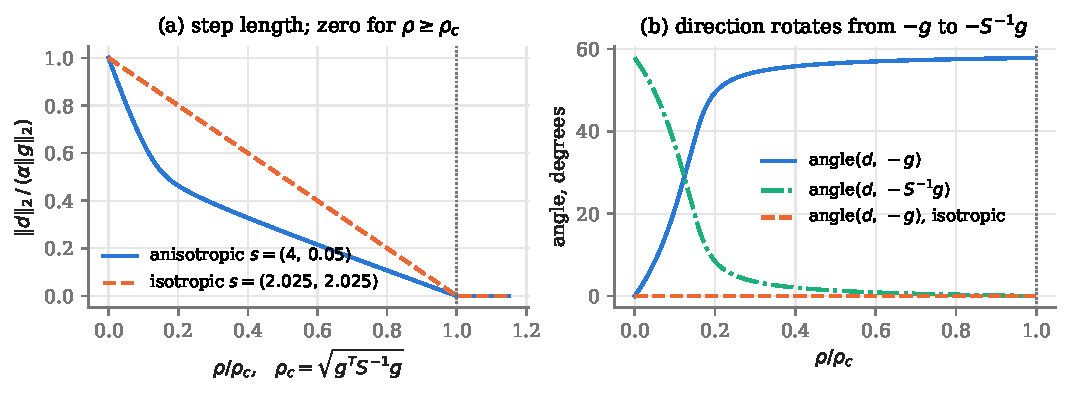
\includegraphics[width=\linewidth]{../fig/zero_step_sweep.pdf}
\caption{Робастный шаг для $g=(1,\,0.6)$, $\alpha=0.5$ как функция $\rho/\rho_c$.
Анизотропная $s=(4,\,0.05)$, $\rho_c=2.73$; изотропная $s$ с тем же средним,
$\rho_c=0.82$. (a) Длина шага относительно SGD; ровно при $\rho=\rho_c$ она становится
нулевой. (b) Угол между $d$ и $-g$ и между $d$ и $-S^{-1}g$; при изотропной $S$
направление не меняется. (Подписи на рисунке на английском.)}
\label{fig:sweep}
\end{figure}

\subsubsection*{Условие оптимальности из 1(d) и независимые проверки}

\begin{center}
\begin{tabular}{@{}p{0.47\linewidth}p{0.45\linewidth}@{}}
\toprule
Проверка & Результат \\
\midrule
Невязка $r(d)$ из 1(d), 20\,000 случайных задач, $m\sim U(0.001,0.999)$ &
$\max r=1.0\cdot10^{-14}$ \\
Невязка на всех траекториях R-SGD из 4.5 & $\max r=9.9\cdot10^{-15}$ \\
Итерации Ньютона, 20\,000 задач &
среднее 4.4, медиана 4, квантиль 99\% — 7, максимум 9 \\
Шаги бисекции / немонотонные итерации Ньютона & $0$ / $0$ (5000 запусков без страховки) \\
Седловая точка (1): $d=-\alpha h^\star$, $h^\star=g+\rho Sd/\sqrt{d^TSd}$ (пункт 1(a)) &
$\max\norm{d+\alpha h^\star}/\norm d=6.0\cdot10^{-12}$ \\
CVXPY (Clarabel), форма SOCP, 300 задач ($s_j$ на четырёх порядках, $m\sim U(0.05,0.95)$) &
наша целевая функция ни разу не больше: $\max(\varphi_{\rm наш}-\varphi_{\rm cvx})/|\varphi|=1.8\cdot10^{-15}$ \\
& $\norm{d-d_{\rm cvx}}/\norm d$: медиана $4.0\cdot10^{-7}$, максимум $4.0\cdot10^{-4}$ \\
Сертификат сильной выпуклости
$\varphi(d+\delta)-\varphi(d)\ge\norm\delta^2/(2\alpha)$, 15\,000 случайных $\delta$ &
наименьший относительный запас $-1.6\cdot10^{-15}$ (только округление) \\
\bottomrule
\end{tabular}
\end{center}

Замечания.
\begin{itemize}
\item Форма SOCP для CVXPY:
$\min_{d,t}\;g^Td+\rho t+\norm d^2/(2\alpha)$ при $\norm{S^{1/2}d}\le t$. Её решения
отличаются от наших до $4\cdot10^{-4}$, потому что метод внутренней точки достигает
точности по целевой функции лишь около $10^{-8}$ (Clarabel пометил 135 из 300 решений как
«optimal\_inaccurate» при запрошенном допуске $10^{-12}$). Так как $\varphi$
$1/\alpha$-сильно выпукла,
$\norm{d_{\rm cvx}-d^\star}^2\le2\alpha(\varphi(d_{\rm cvx})-\varphi(d^\star))$, и разрыв
$10^{-8}$ по целевой функции объясняет расстояние $10^{-4}$. Наша целевая функция ни
разу не оказалась больше, чем у CVXPY.
\item Тест сертификата — прямое доказательство оптимальности: для точного минимума
$1/\alpha$-сильно выпуклой функции неравенство выполнено при любом $\delta$, а в
неоптимальной точке оно нарушается для малых $\delta$ вдоль направления убывания.
\item Ошибка седловой точки — это та же невязка, измеренная иначе:
$d+\alpha h^\star=\alpha\,(g+\rho Sd/\tau+d/\alpha)$, поэтому она умножена на
$\alpha\norm g/\norm d$, что велико чуть ниже порога.
\end{itemize}

\subsubsection*{Нулевые шаги на траекториях зашумлённой квадратичной задачи}

Это иллюстрация, а не настроенное сравнение: $b=8$, $\alpha_0=0.2$ (меньше
$2/L=0.5$), $\alpha_k=\alpha_0/\sqrt{1+k/50}$, $K=300$ обновлений, $\theta_0=(2,2)$,
20 сидов с общими случайными числами (оба метода получают одни и те же $z_{k,i}$),
$\rho\in\{1,\,2.45\}$. Значение $2.45\approx\sqrt{\chi^2_{2,0.95}}$ — радиус, при
котором при большом $b$ 95\% обновлений в точке минимума оказываются нулевыми (раздел~\ref{sec:batch}).

\begin{center}
\small
\begin{tabular}{@{}llcccc@{}}
\toprule
$\sigma$ & метод & \shortstack{медиана итогового\\ $f$ [IQR]} & \shortstack{нулевые\\ шаги} & \shortstack{макс.\ $f$ при\\ нулевом шаге} & \shortstack{ср.\ итераций\\ Ньютона} \\
\midrule
0 & SGD & $6.3\cdot10^{-31}$ & -- & -- & -- \\
0 & R-SGD $\rho=1$ & $5.0\cdot10^{-12}$ & 0 & -- & 1.0 \\
0 & R-SGD $\rho=2.45$ & $3.0\cdot10^{-11}$ & 0 & -- & 1.0 \\
\midrule
1 & SGD & $0.0034$ [0.0020, 0.0067] & -- & -- & -- \\
1 & R-SGD $\rho=1$ & $0.0016$ [0.0005, 0.0073] & 33.0\% & 0.94 & 4.3 \\
1 & R-SGD $\rho=2.45$ & $0.0196$ [0.0085, 0.0386] & 80.8\% & 1.59 & 4.1 \\
\midrule
4 & SGD & $0.054$ [0.033, 0.107] & -- & -- & -- \\
4 & R-SGD $\rho=1$ & $0.026$ [0.008, 0.116] & 33.7\% & 2.50 & 4.3 \\
4 & R-SGD $\rho=2.45$ & $0.126$ [0.027, 0.269] & 85.0\% & 2.94 & 3.9 \\
\bottomrule
\end{tabular}
\end{center}
(IQR — интерквартильный размах по 20 сидам.)

\begin{figure}[H]
\centering
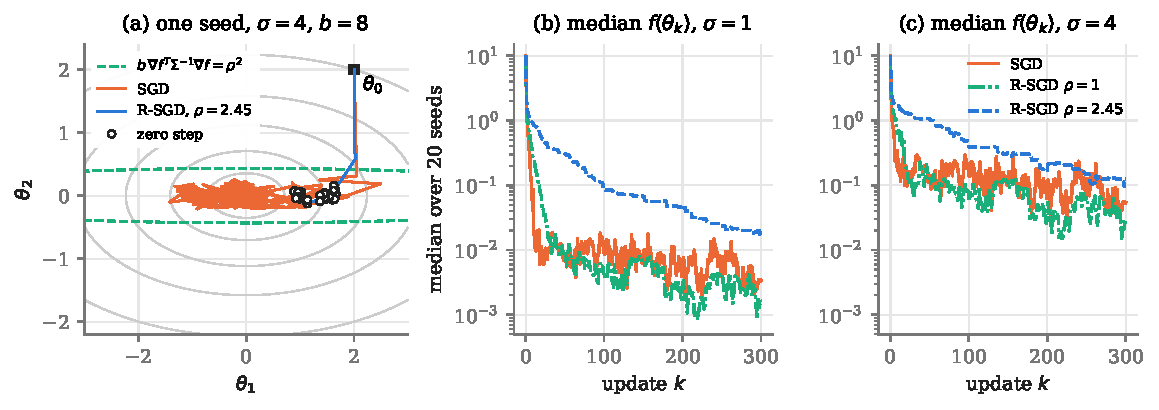
\includegraphics[width=\linewidth]{../fig/quadratic_trajectories.pdf}
\caption{Зашумлённая квадратичная задача, $b=8$, $\alpha_0=0.2$, 300 обновлений.
(a) Один сид при $\sigma=4$: SGD и R-SGD ($\rho=2.45$) с одинаковыми реализациями шума;
кружки отмечают точки, где R-SGD сделал нулевой шаг; пунктирный эллипс —
$b\,\nabla f^T\Sigma^{-1}\nabla f=\rho^2$ (полуоси $6.9$ и $0.43$, поэтому в этом окне он
выглядит как горизонтальная полоса). (b), (c) Медиана $f(\theta_k)$ по 20 сидам.}
\label{fig:traj}
\end{figure}

Что показывают эти числа:
\begin{itemize}
\item \textbf{Нулевые шаги происходят далеко от минимума.} При $\sigma=4$,
$\rho=2.45$ нулевые шаги случались в точках с $f$ до $2.94$ (при $f(\theta_0)=10$ и
$f^\star=0$), где $\norm{\nabla f}$ далеко не ноль. Рис.~\ref{fig:traj}(a) объясняет
почему: вдоль $\theta_1$ градиент $\theta_1$ слабый, а шум сильный (стандартное
отклонение $2\sigma$ на наблюдение), поэтому ожидаемая статистика
$b\,\nabla f^T\Sigma^{-1}\nabla f=b\big(\theta_1^2/(4\sigma^2)+64\theta_2^2/\sigma^2\big)$
остаётся меньше $\rho^2$ при $|\theta_1|$ вплоть до $\rho\cdot2\sigma/\sqrt b=6.9$.
R-SGD быстро исправляет $\theta_2$, где отношение сигнал/шум велико, а затем
останавливается по $\theta_1$. Это численное подтверждение ответа на 1(c): из (3) не
следует $\nabla f(\theta_k)=0$.
\item \textbf{Добавка $\varepsilon_k$ при $\sigma=0$.} Все наблюдения совпадают,
$S_k=10^{-11}I$, и R-SGD сходится к границе своей области нулевого шага
$\norm{\nabla f}=\rho\sqrt{\varepsilon}$, где
$f\approx\norm{\nabla f}^2/2=\rho^2\varepsilon/2$: $5.0000\cdot10^{-12}$ при $\rho=1$
и $3.0013\cdot10^{-11}$ при $\rho=2.45$, что совпадает с измеренными медианами до
девяти знаков. Приближение к границе непрерывно, поэтому ни одного точного нулевого шага
не зафиксировано. Так как $S=\varepsilon I$ изотропна, Ньютон на каждом обновлении
делал одну итерацию.
\item \textbf{Умеренный радиус может помочь, большой — тормозит.} $\rho=1$ уменьшил
медиану итогового $f$ (0.0016 против 0.0034 при $\sigma=1$; 0.026 против 0.054 при
$\sigma=4$), но интерквартильные размахи перекрываются, а $\rho=2.45$ оказался хуже SGD
при обоих уровнях шума. Это ненастроенные иллюстративные запуски; сохранится ли выигрыш
при честной настройке $\alpha_0$ для обоих методов и сводится ли он к укорочению шага —
рассматривается в разделах~\ref{sec:protocol}--\ref{sec:critical}.
\item \textbf{Стоимость.} Оба метода потратили $2400=bK$ вычислений градиента за
запуск; время — около 4--7\,мс на запуск для SGD и 9--23\,мс для R-SGD (запуски с
большим числом нулевых шагов быстрее, так как нулевой шаг не вызывает Ньютона).
\end{itemize}

\subsection{(c) Размер батча и оценка неопределённости}\label{sec:batch}

\subsubsection*{Теория}

Зафиксируем $\theta$ и будем считать наблюдения гауссовскими, как в квадратичной задаче:
$v_{i,j}\sim\mathcal N(\mu_j,\Sigma_{jj})$ независимо, с независимыми координатами
($A$ диагональна). Из стандартных фактов о гауссовских выборках следует:
\begin{enumerate}
\item \textbf{Среднее.} $\E\widehat s_j=\Sigma_{jj}/b$ (раздел~\ref{sec:S}): сама оценка убывает как
$1/b$, потому что она оценивает дисперсию среднего.
\item \textbf{Разброс.} $(b-1)\,b\,\widehat s_j/\Sigma_{jj}\sim\chi^2_{b-1}$, отсюда
$\operatorname{sd}(\widehat s_j)/\E\widehat s_j=\sqrt{2/(b-1)}$: 141\% при $b=2$, 53\%
при $b=8$, 9\% при $b=256$. При маленьком батче сама $S_k$ очень шумная.
\item \textbf{Статистика нулевого шага.} $g_j$ и $\widehat s_j$ независимы, и
$\E[1/\chi^2_\nu]=1/(\nu-2)$, поэтому (без учёта $\varepsilon_k$)
\begin{align*}
\E\big[g^TS^{-1}g\big]&=\sum_j\E[g_j^2]\,\E[1/\widehat s_j]
=\sum_j\Big(\mu_j^2+\frac{\Sigma_{jj}}b\Big)\frac{b}{\Sigma_{jj}}\,\frac{b-1}{b-3}\\
&=\big(b\,\mu^T\Sigma^{-1}\mu+p\big)\frac{b-1}{b-3},\qquad b>3 .
\end{align*}
Вдали от стационарной точки ($\mu\ne0$) статистика растёт \emph{линейно} по $b$,
поэтому при фиксированном $\rho$ нулевые шаги с ростом $b$ исчезают. В стационарной
точке ($\mu=0$) каждое $g_j/\sqrt{\widehat s_j}$ имеет распределение Стьюдента с $b-1$
степенями свободы, среднее равно $p(b-1)/(b-3)$, а при $b\le3$ оно бесконечно (тяжёлые
хвосты). При больших $b$ $g^TS^{-1}g\to\chi^2_p$ по распределению, что задаёт
естественный масштаб для $\rho$: $\rho=\sqrt{\chi^2_{p,0.95}}$ ($=2.45$ при $p=2$)
означает 95\% нулевых шагов в точке минимума.
\item \textbf{Величина робастной поправки.} Радиус неопределённости в единицах
градиента $\rho\sqrt{s_j}\propto\rho/\sqrt b$, поэтому коэффициенты сжатия из 2.7
стремятся к 1, и при фиксированном $\rho$ и $b\to\infty$ R-SGD переходит в SGD. Иначе
говоря, $\rho$ и $b$ — не независимые параметры: один и тот же $\rho$ означает разную
степень робастности при разных размерах батча.
\end{enumerate}

\subsubsection*{Численная проверка}

$\sigma=1$ (так что $\Sigma=\diag(4,\tfrac14)$), $20\,000$ независимых батчей для
каждого $b$, в трёх фиксированных точках: минимум $\theta^\star=(0,0)$, промежуточная
точка $\theta_{\rm mid}=(1,\,0.1)$ с $\mu^T\Sigma^{-1}\mu=0.89$ и $\theta_0=(2,2)$ с
$\mu^T\Sigma^{-1}\mu=257$. Нулевые шаги считаются при $\rho=2.45$; последний столбец —
среднее относительное изменение шага $\norm{d+\alpha g}/(\alpha\norm g)$ в
$\theta_{\rm mid}$ при $\rho=1$, $\alpha=0.1$.

\begin{center}
\small
\setlength{\tabcolsep}{4.0pt}
\begin{tabular}{@{}rccccccccc@{}}
\toprule
& \multicolumn{2}{c}{$b\,\E\widehat s_j/\Sigma_{jj}$} & \multicolumn{2}{c}{отн.\ разброс $\widehat s_1$}
& \multicolumn{2}{c}{$\E\,g^TS^{-1}g$ в $\theta^\star$} & \multicolumn{2}{c}{доля нулевых шагов} & отн.\ изм. \\
\cmidrule(lr){2-3}\cmidrule(lr){4-5}\cmidrule(lr){6-7}\cmidrule(lr){8-9}
$b$ & $j=1$ & $j=2$ & эмп. & $\sqrt{2/(b-1)}$ & эмп. & теория & $\theta^\star$ & $\theta_{\rm mid}$ & в $\theta_{\rm mid}$ \\
\midrule
2 & 1.002 & 1.013 & 1.415 & 1.414 & 788.47 & $\infty$ & 0.558 & 0.410 & 0.579 \\
3 & 0.998 & 1.011 & 1.011 & 1.000 & 13.27 & $\infty$ & 0.719 & 0.484 & 0.606 \\
4 & 1.003 & 1.000 & 0.819 & 0.816 & 5.32 & 6.00 & 0.794 & 0.479 & 0.604 \\
8 & 0.994 & 0.999 & 0.534 & 0.535 & 2.78 & 2.80 & 0.885 & 0.297 & 0.536 \\
16 & 0.999 & 1.003 & 0.365 & 0.365 & 2.30 & 2.31 & 0.922 & 0.076 & 0.441 \\
32 & 0.998 & 1.003 & 0.251 & 0.254 & 2.14 & 2.14 & 0.938 & 0.001 & 0.338 \\
64 & 1.001 & 0.998 & 0.178 & 0.178 & 2.04 & 2.07 & 0.946 & 0.000 & 0.237 \\
128 & 0.999 & 1.000 & 0.126 & 0.125 & 2.02 & 2.03 & 0.946 & 0.000 & 0.167 \\
256 & 1.001 & 1.000 & 0.089 & 0.089 & 1.99 & 2.02 & 0.952 & 0.000 & 0.117 \\
\bottomrule
\end{tabular}
\end{center}
В точке $\theta_0$ доля нулевых шагов была равна $0$ при всех $b$.

\begin{figure}[H]
\centering
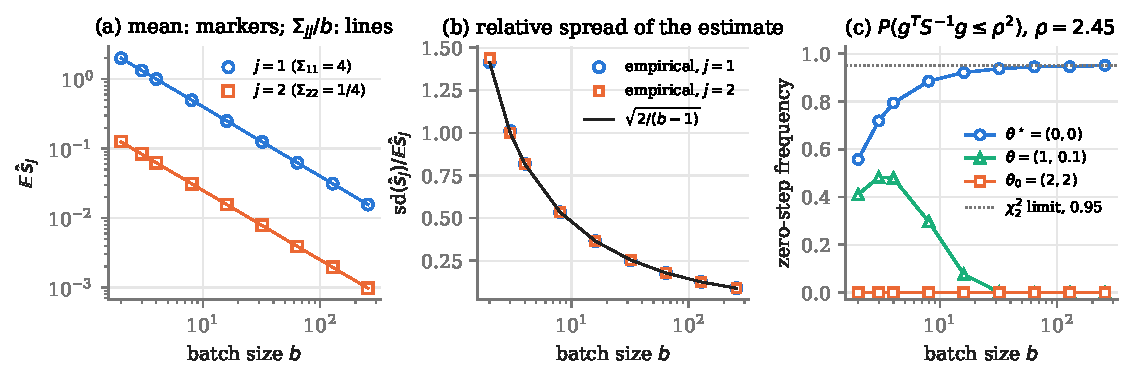
\includegraphics[width=\linewidth]{../fig/batch_size.pdf}
\caption{Размер батча и оценка неопределённости (квадратичная задача, $\sigma=1$,
$20\,000$ батчей на каждое $b$). (a) $\E\widehat s_j$ следует $\Sigma_{jj}/b$.
(b) Относительный разброс следует $\sqrt{2/(b-1)}$. (c) Доля нулевых шагов при
$\rho=2.45$ в трёх точках; в $\theta^\star$ она стремится к значению $0.95$ для
$\chi^2_2$.}
\label{fig:batch}
\end{figure}

Как читать результаты:
\begin{itemize}
\item Пункты 1 и 2 из 5.1 подтверждаются в пределах ошибки Монте-Карло при всех $b$
(отношения $1.00\pm0.013$; разброс отличается от $\sqrt{2/(b-1)}$ не более чем на
$0.025$).
\item Среднее $g^TS^{-1}g$ в $\theta^\star$ совпадает с $p(b-1)/(b-3)$ при $b\ge8$.
При $b=2,3$ теоретическое среднее бесконечно, и выборочные средние (788 и 13) ничего не
значат; при $b=4$ бесконечна дисперсия статистики, поэтому выборочное среднее сходится
медленно (5.3 против 6.0). Это эффект тяжёлых хвостов оценки дисперсии по двум-трём
точкам.
\item В $\theta_{\rm mid}$ доля нулевых шагов падает примерно с $0.4$--$0.5$ до $0$
между $b=4$ и $b=32$: переход происходит там, где $b\,\mu^T\Sigma^{-1}\mu\approx\rho^2$,
то есть при $b\approx6/0.89\approx7$. При $b\le4$ доля \emph{не} монотонна: при очень
маленьком батче $\widehat s_j$ часто случайно оказывается крошечной, $g^TS^{-1}g$
резко растёт, и нулевого шага не происходит. Поэтому решения о нулевом шаге при $b\le4$
в значительной степени случайны.
\item Робастная поправка убывает как $1/\sqrt b$: от $b=64$ к $b=256$ относительное
изменение уменьшается вдвое ($0.237\to0.117$). При фиксированном $\rho$ R-SGD с большим
$b$ почти совпадает с SGD.
\end{itemize}

\subsubsection*{Почему выбор с возвращением}

В обучаемых моделях наблюдения берутся из конечной обучающей выборки размера $n$. С
возвращением $b$ выборок независимы и одинаково распределены, и
$\E\widehat s_j=\Var(g_j)$ точно. Без возвращения дисперсия среднего по батчу получает
множитель конечной совокупности $(n-b)/(n-1)$, а выборочная дисперсия по-прежнему
оценивает дисперсию совокупности, поэтому $\widehat s_j$ завышает $\Var(g_j)$ в
$n/(n-b)$ раз. Проверка на данных логистической регрессии с $n=64$, $\sigma=0$,
$20\,000$ батчей:

\begin{center}
\begin{tabular}{@{}ccccc@{}}
\toprule
$n$ & $b$ & $\E\widehat s_j/\Var(g_j)$, с возвр. & без возвр. & прогноз $n/(n-b)$ \\
\midrule
64 & 8 & 1.000--1.002 & 1.139--1.143 & 1.143 \\
64 & 32 & 0.999--1.003 & 2.000--2.004 & 2.000 \\
\bottomrule
\end{tabular}
\end{center}
(Диапазоны — по трём координатам $w_1,w_2,c$.) Без возвращения при $b=n/2$
неопределённость была бы завышена вдвое, что приводило бы к ложным нулевым шагам.

\subsection{(d) Решения, необходимые для воспроизведения}\label{sec:repro2}

\begin{itemize}
\item \textbf{Код.} \texttt{rsgd.py} (оценка (4), решатель, цикл SGD/R-SGD, оракулы,
генераторы данных, проверка конечными разностями) и \texttt{checks\_section2.py} (все
числа, таблицы и рисунки этого раздела). Запуск: \texttt{python checks\_section2.py};
полный прогон занимает около 20\,с.
\item \textbf{Случайные числа.} Один главный сид $20261117$; эксперименты используют
независимые дочерние потоки \texttt{numpy.random.SeedSequence(20261117).spawn(8)}.
Внутри одного запуска оптимизации два отдельных генератора: для индексов батча и для
шума градиента $z_{k,i}$ (в разделе~\ref{sec:sims} ещё по одному для данных и для инициализации).
\item \textbf{Общие случайные числа.} SGD и R-SGD запускаются со свежими генераторами с
одинаковыми сидами, поэтому в парном сравнении они получают одни и те же индексы батчей и
одни и те же $z_{k,i}$ на каждой итерации (наблюдения всё же различаются, как только
расходятся итерации, поскольку $u_i$ вычисляется в разных $\theta_k$).
\item \textbf{Модель искажения.} Шум добавляется только к наблюдениям $V$. Целевая
функция $f$, обучающие данные, все потери и точности вычисляются на чистых данных.
\item \textbf{Настройки.} Везде float64; $b$, $\alpha_0$, расписание
$\alpha_0/\sqrt{1+k/50}$, число обновлений $K$, $\rho$, $\sigma$, $\theta_0$ — как указано
в каждой проверке; $\varepsilon_k$ строго по (4); допуски решателя $|\psi|\le10^{-14}$,
относительный шаг $\le10^{-15}$, не более 100 итераций; нулевой шаг фиксируется только
при $g^TS^{-1}g\le\rho^2$.
\item \textbf{Что сохраняется для каждого запуска.} Число вычислений градиента ($bK$ для
обоих методов), время, число нулевых шагов, итерации Ньютона, максимальная невязка 1(d).
\item \textbf{ПО.} Python 3.13.18, NumPy 2.5.3, SciPy 1.18.1, Matplotlib 3.11.2,
CVXPY 1.9.3 (Clarabel) — только для перекрёстной проверки.
\end{itemize}

\section{Обязательные эксперименты}\label{sec:sims}

Оба эксперимента сравнивают SGD и R-SGD по протоколу раздела~\ref{sec:protocol}. Выбранные там и
затем зафиксированные для всех уровней шума настройки:
\begin{itemize}
\item логистическая регрессия: SGD $\alpha_0=0.3$; R-SGD $\alpha_0=1$, $\rho=0.75\sqrt3=1.30$;
\item сеть: SGD $\alpha_0=1$; R-SGD $\alpha_0=10$, $\rho=0.25\sqrt{33}=1.44$.
\end{itemize}
Все числа получены скриптом \texttt{sim\_section3.py} (\texttt{results\_section3.json}), все
таблицы — скриптом \texttt{make\_tables3.py}.

\subsection{Общие условия}\label{sec:setup}


\begin{center}
\small
\begin{tabular}{@{}p{0.27\linewidth}p{0.68\linewidth}@{}}
\toprule
Элемент & Выбор и причина \\
\midrule
Данные & сбалансированные классы; $n_{\rm train}=400$, $n_{\rm val}=400$, $n_{\rm test}=4000$,
выбираются независимо (большая тестовая выборка: стандартная ошибка точности $\le0.005$) \\
Предобработка & стандартизация $a\mapsto(a-\bar a_{\rm train})/s_{\rm train}$ по среднему и
стандартному отклонению \emph{только обучающей} выборки, применяется ко всем трём выборкам \\
Потери & $\ell(t,y)=\log(1+e^t)-yt$, вычисляются как \texttt{logaddexp(0,t)-y*t}; цель —
средние потери на обучении без регуляризатора; класс $=\mathbf 1[t>0]$ \\
Батч и бюджет & $b=16$, выбор с возвращением; $K=500$ обновлений (логистическая), $K=3000$
(сеть); $bK$ вычислений градиента за запуск у обоих методов \\
Шаги & $\alpha_k=\alpha_0/\sqrt{1+k/50}$ для обоих методов \\
Шум градиента & $v_{k,i}=u_i(\theta_k)+\sigma z_{k,i}$, $z_{k,i}\sim\mathcal N(0,I_p)$, независимы
по наблюдениям и итерациям; $\sigma=c\,\gamma$, $c\in\{0,1,4,16\}$ \\
Единица шума $\gamma$ & среднеквадратичное значение чистых градиентов примеров в начальной
точке, усреднённое по сидам настройки: $\gamma=0.500$ (логистическая), $\gamma=0.215$ (сеть) \\
Модель неопределённости & $g_k$, $S_k$ по формуле (4) из \emph{тех же} $b$ наблюдений, что
используются в обновлении \\
Оценка & все потери и точности на чистых данных; 61 контрольная точка на запуск для кривых \\
\bottomrule
\end{tabular}
\end{center}

\textbf{Уровни шума.} $c=0$ — случай без искусственного искажения (только шум выбора
мини-батча). При $c=1$ искажение одного наблюдения сравнимо с типичной координатой градиента
примера. При $c=4$ и $c=16$ оно доминирует. После усреднения по $b=16$ наблюдениям добавленный
шум в $g_k$ имеет стандартное отклонение $c\gamma/4$ на координату.

\textbf{Масштаб радиуса.} Радиус параметризуется как $\rho=r\sqrt p$. Вблизи стационарной
точки $g_k^TS_k^{-1}g_k$ приближённо распределено как $\chi^2_p$ со средним $p(b-1)/(b-3)$
(раздел~\ref{sec:batch}), поэтому порог правила нулевого шага растёт как $\sqrt p$. Фиксированное
$\rho$ означало бы совсем разное при $p=3$ и $p=33$; в терминах $r$ смысл одинаков: $r\approx1$
— точка, с которой вблизи минимума начинаются нулевые шаги.

\subsection{Эксперимент 1: логистическая регрессия}\label{sec:sim1}

\subsubsection*{Модель, градиент и эталон}

$a\mid y\sim\mathcal N\big((2y-1)(1,1)^T,I_2\big)$, $t_\theta(a)=w^Ta+c$, $\theta=(w_1,w_2,c)$,
$p=3$, $\theta_0=0$ (задача выпукла, поэтому фиксированная начальная точка естественна).
Градиент примера $u_i(\theta)=(\sigm(t_i)-y_i)\,(a_i^T,1)^T$ (раздел~\ref{sec:oracles}). Проверка
конечными разностями на данных оценки даёт относительные ошибки $2.7\cdot10^{-10}$ (средний
градиент) и $1.9\cdot10^{-10}$ (по примерам).

\textbf{Эталон.} Модель корректно специфицирована: логарифм отношения правдоподобий
$\log\frac{p(a\mid1)}{p(a\mid0)}=2\,(1,1)a$, поэтому байесовское правило — $a_1+a_2>0$ с
точностью $\Phi(\sqrt2)\approx0.921$. На фактических тестовых выборках схемы A байесовское
правило имеет точность $0.9228\pm0.0031$ и потери $0.1905\pm0.0065$ (истинный логит
$2(a_1+a_2)$). В среднем ни один метод не может быть лучше.

\subsubsection*{Результаты}

\begin{figure}[H]
\centering
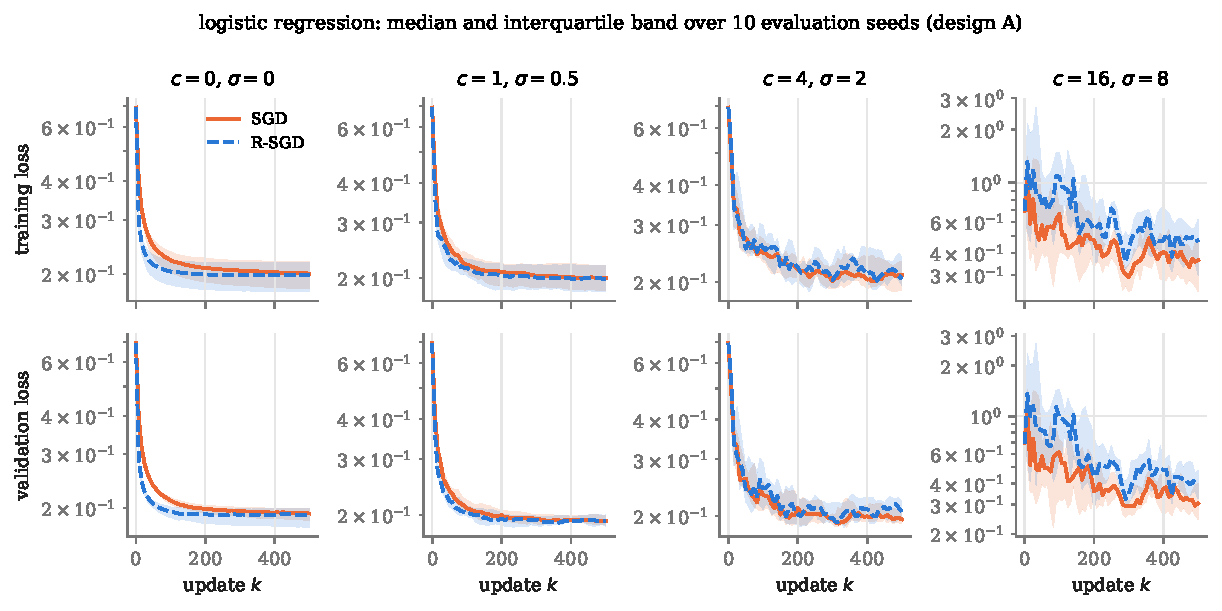
\includegraphics[width=\linewidth]{../fig3/logreg_curves.pdf}
\caption{Логистическая регрессия: потери на обучении (сверху) и на валидации (снизу) на чистых
данных в зависимости от номера обновления; медиана и интерквартильная полоса по 10 сидам оценки
(схема A). Зафиксированные настройки: SGD $\alpha_0=0.3$; R-SGD $\alpha_0=1$, $\rho=1.30$.}
\label{fig:lr_curves}
\end{figure}

\begin{center}
\small
\setlength{\tabcolsep}{4pt}
\begin{tabular}{@{}clccccc@{}}
\toprule
$c$ & метод & \shortstack{итог.\ потери\\обуч.} & \shortstack{потери\\на тесте} & \shortstack{точность\\на тесте} & \shortstack{нулевые\\шаги} & \shortstack{время, мс\\(мкс/обн.)} \\
\midrule
\tabinput{../tabs3/tab_lr_main.tex}
\bottomrule
\end{tabular}

\smallskip
Логистическая регрессия, схема A, среднее $\pm$ sd по 10 сидам; $bK=8000$ вычислений градиента
за запуск у обоих методов; байесовское правило: точность $0.9228$, потери на тесте $0.1905$.
\end{center}

\begin{center}
\footnotesize
\setlength{\tabcolsep}{2.6pt}
\begin{tabular}{@{}cccccccccc@{}}
\toprule
& & \multicolumn{2}{c}{$\Delta$ потерь обуч.} & \multicolumn{2}{c}{$\Delta$ потерь на тесте}
& \multicolumn{2}{c}{$\Delta$ точности} & \multicolumn{2}{c}{совпадение} \\
\cmidrule(lr){3-4}\cmidrule(lr){5-6}\cmidrule(lr){7-8}\cmidrule(lr){9-10}
$c$ & схема & среднее $\pm$ h & побед & среднее $\pm$ h & побед & среднее $\pm$ h & \shortstack{побед\\(ничьи)} & \shortstack{об.$\to$\\тест} & \shortstack{об.$\to$\\точн.} \\
\midrule
\tabinput{../tabs3/tab_lr_paired.tex}
\bottomrule
\end{tabular}

\smallskip
Парные разности R-SGD $-$ SGD (отрицательная разность потерь и положительная разность точности
в пользу R-SGD); «совпадение ранжирования» — число сидов, в которых знак $\Delta$ потерь на
обучении предсказывает знак $\Delta$ потерь на тесте (об.$\to$тест) или $-\Delta$ точности
(об.$\to$точн.).
\end{center}

Как читать результаты.
\begin{itemize}
\item \textbf{Точность насыщена.} При $c\le4$ оба метода отстоят от байесовской точности не
более чем на $0.005$, а средняя разность точностей по модулю меньше $0.001$. Разности потерь в
несколько тысячных сдвигают линейную границу пренебрежимо мало (рис.~\ref{fig:lr_bound}).
\item \textbf{Малый, но устойчивый выигрыш по потерям при $c\le1$.} На фиксированном наборе
данных (схема B) у R-SGD меньше потери на обучении в 10/10 ($c=0$) и 9/10 ($c=1$) сидов и
меньше потери на тесте в 10/10 и 8/10. При смене наборов данных (схема A) те же разности
скрываются гораздо большим разбросом между наборами (sd потерь на тесте $0.007$ в A против
$0.001$ в B при $c=0$).
\item \textbf{Хуже при $c\ge4$ с зафиксированными настройками.} R-SGD работает с
$\alpha_0=1$, втрое большим, чем у SGD, и полагается на сжатие как на компенсацию. Когда шум
доминирует, сжатие почти постоянно (раздел~\ref{sec:critical}(a)), большие шумные градиенты проходят, и потери выше:
$+0.005$ при $c=4$ и $+0.095$ при $c=16$; SGD лучше в 7--8 из 10 сидов.
\item \textbf{Нулевые шаги:} 18\% обновлений при $c=0$ и 32--33\% при $c\ge1$, включая
обновления в начале обучения. Они не помешали сходимости, поскольку $p=3$, а остальные шаги
большие.
\item \textbf{Время:} SGD 16--21\,мкс на обновление, R-SGD 58--88\,мкс (в 2.8--4.4 раза больше)
при одинаковом числе вычислений градиента.
\end{itemize}

\begin{figure}[H]
\centering
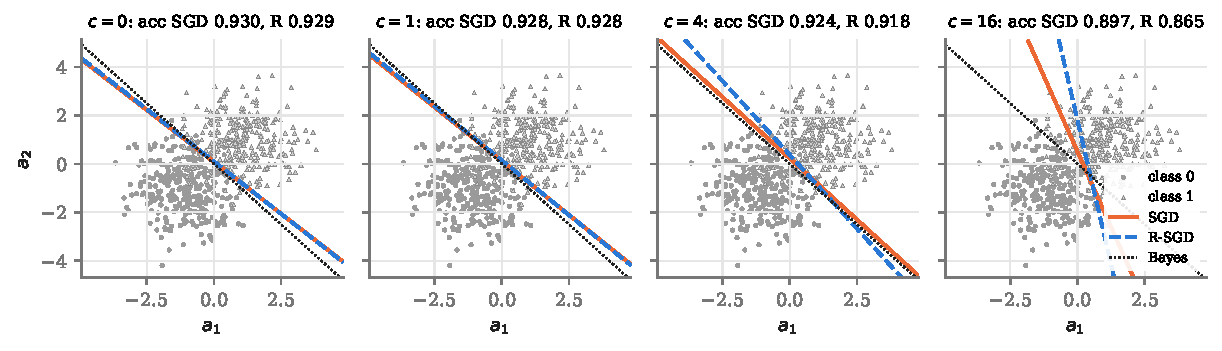
\includegraphics[width=\linewidth]{../fig3/logreg_boundaries.pdf}
\caption{Логистическая регрессия, сид оценки A-0 (сиды указаны в разделе~\ref{sec:repro}): границы решения
$t_\theta(a)=0$ итоговых точек SGD и R-SGD в исходных координатах, байесовская граница
$a_1+a_2=0$ и 600 тестовых точек.}
\label{fig:lr_bound}
\end{figure}

\subsection{Эксперимент 2: двухслойная сеть}\label{sec:sim2}

\subsubsection*{Модель, инициализация, градиент}

Полуокружности: $t\sim U[0,\pi]$, класс 0 в точке $(\cos t,\sin t)+e$, класс 1 в точке
$(1-\cos t,\tfrac12-\sin t)+e$, $e\sim\mathcal N(0,0.1^2I_2)$. Модель
$t_\theta(a)=w_2^T\tanh(W_1a+b_1)+b_2$ с 8 скрытыми нейронами, $p=33$. Инициализация:
$W_1\sim\mathcal N(0,\tfrac12)$, $b_1=0$, $w_2\sim\mathcal N(0,\tfrac18)$, $b_2=0$ (дисперсия
$1/\text{fan-in}$), из потока инициализации данного сида; SGD и R-SGD стартуют из одной и той же
$\theta_0$. Начальные потери близки к $\log2=0.693$. Градиент вычисляется обратным
распространением по каждому примеру (раздел~\ref{sec:oracles}); проверка конечными разностями в
фактической начальной точке даёт относительные ошибки $4.9\cdot10^{-10}$ (средний) и
$8.9\cdot10^{-10}$ (по примерам).

\subsubsection*{Результаты}

\begin{figure}[H]
\centering
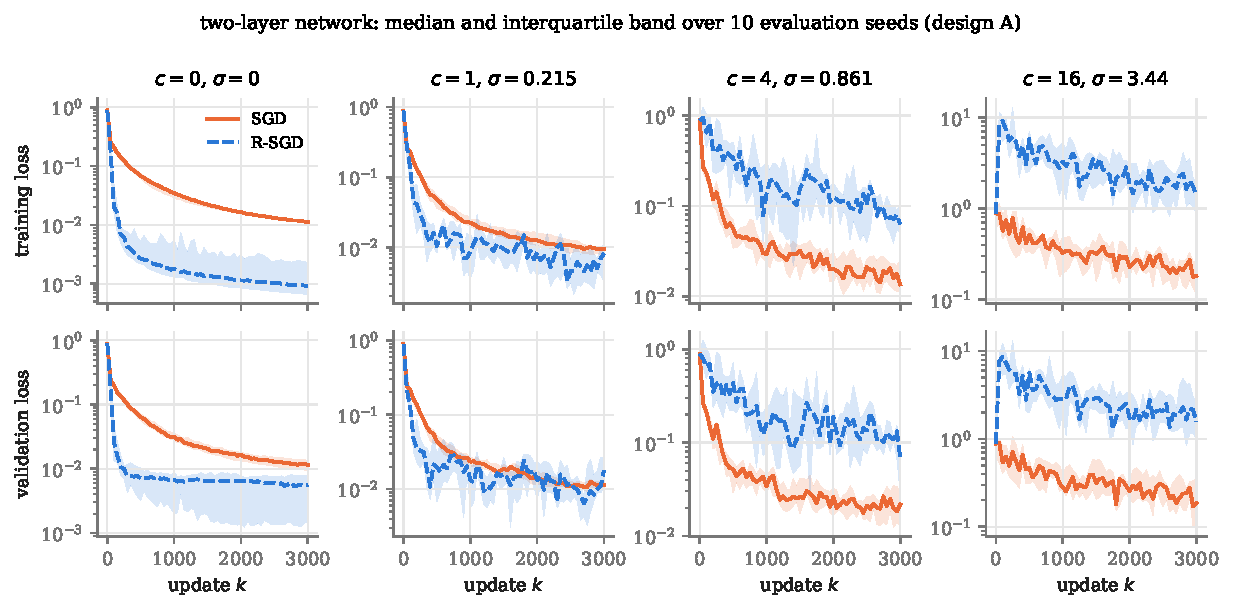
\includegraphics[width=\linewidth]{../fig3/mlp_curves.pdf}
\caption{Двухслойная сеть: потери на обучении (сверху) и на валидации (снизу) на чистых
данных, медиана и интерквартильная полоса по 10 сидам оценки (схема A). Зафиксированные
настройки: SGD $\alpha_0=1$; R-SGD $\alpha_0=10$, $\rho=1.44$.}
\label{fig:mlp_curves}
\end{figure}

\begin{center}
\small
\setlength{\tabcolsep}{4pt}
\begin{tabular}{@{}clccccc@{}}
\toprule
$c$ & метод & \shortstack{итог.\ потери\\обуч.} & \shortstack{потери\\на тесте} & \shortstack{точность\\на тесте} & \shortstack{нулевые\\шаги} & \shortstack{время, мс\\(мкс/обн.)} \\
\midrule
\tabinput{../tabs3/tab_mlp_main.tex}
\bottomrule
\end{tabular}

\smallskip
Двухслойная сеть, схема A, среднее $\pm$ sd по 10 сидам; $bK=48\,000$ вычислений градиента за
запуск у обоих методов.
\end{center}

\begin{center}
\footnotesize
\setlength{\tabcolsep}{2.6pt}
\begin{tabular}{@{}cccccccccc@{}}
\toprule
& & \multicolumn{2}{c}{$\Delta$ потерь обуч.} & \multicolumn{2}{c}{$\Delta$ потерь на тесте}
& \multicolumn{2}{c}{$\Delta$ точности} & \multicolumn{2}{c}{совпадение} \\
\cmidrule(lr){3-4}\cmidrule(lr){5-6}\cmidrule(lr){7-8}\cmidrule(lr){9-10}
$c$ & схема & среднее $\pm$ h & побед & среднее $\pm$ h & побед & среднее $\pm$ h & \shortstack{побед\\(ничьи)} & \shortstack{об.$\to$\\тест} & \shortstack{об.$\to$\\точн.} \\
\midrule
\tabinput{../tabs3/tab_mlp_paired.tex}
\bottomrule
\end{tabular}

\smallskip
Двухслойная сеть: парные разности R-SGD $-$ SGD, как в таблице для логистической регрессии.
\end{center}

Как читать результаты.
\begin{itemize}
\item \textbf{$c=0$: R-SGD оптимизирует быстрее.} Потери на обучении $0.0019$ против
$0.0110$ (10/10 сидов в обеих схемах); потери на тесте меньше в 9/10 (A) и 10/10 (B). Кривые на
рис.~\ref{fig:mlp_curves} расходятся через несколько сотен обновлений. Точность не лучше
(3 победы, 2 ничьи), так как оба метода уже правильно классифицируют $99.8\%$ тестовых точек.
\item \textbf{Выигрыш при $c=0$ — выигрыш длины шага.} Среднее отношение шагов R-SGD $0.59$,
поэтому он движется как SGD с $\alpha_0'=5.9$, в шесть раз большим настроенного для SGD $1$. Такой
SGD достигает потерь на тесте $0.0065$ против $0.0082$ у R-SGD (R-SGD лучше в 4/10). Значение
$\alpha_0=1$ для SGD выбрано при $c=1$ по шумному критерию, а не при $c=0$.
\item \textbf{$c=1$, сам уровень настройки: R-SGD хуже.} Потери на валидации при оценке
$0.0230\pm0.0207$ против $0.0114\pm0.0028$ у SGD, хотя настройка предсказывала обратное
($0.0104$ против $0.0138$). Выбор R-SGD — минимум по 36 шумным оценкам против 6 у SGD, поэтому он
смещён в оптимистичную сторону («проклятие победителя»), а выбранный большой $\alpha_0=10$ —
настройка с большой дисперсией. Точность на тесте $0.9946$ против $0.9980$; SGD лучше в 8 из 10
сидов (одна ничья).
\item \textbf{$c\ge4$: зафиксированная настройка R-SGD разваливается.} Потери на тесте $0.115$
против $0.025$ ($c=4$) и $1.96$ против $0.22$ ($c=16$); при $c=16$ 8 из 10 запусков R-SGD
заканчиваются потерями на обучении выше начальных $\log2$. Эффективный шаг около
$7.4/\sqrt{1+k/50}$, то есть в 7.4 раза больше, чем у SGD, при градиентах, в которых доминирует
шум, выбрасывает сеть в области насыщения. Ни один запуск не попал под формальный критерий
неудачи (потери $>50$ начальных).
\item \textbf{Нулевые шаги:} при выбранном $\rho=1.44$ их нет: это намного меньше порога для
режима доминирующего шума $\approx\sqrt{p(b-1)/(b-3)}=6.2$.
\item \textbf{Время:} SGD 32--49\,мкс на обновление, R-SGD 109--128\,мкс (в 2.6--3.6 раза
больше).
\end{itemize}

\begin{figure}[H]
\centering
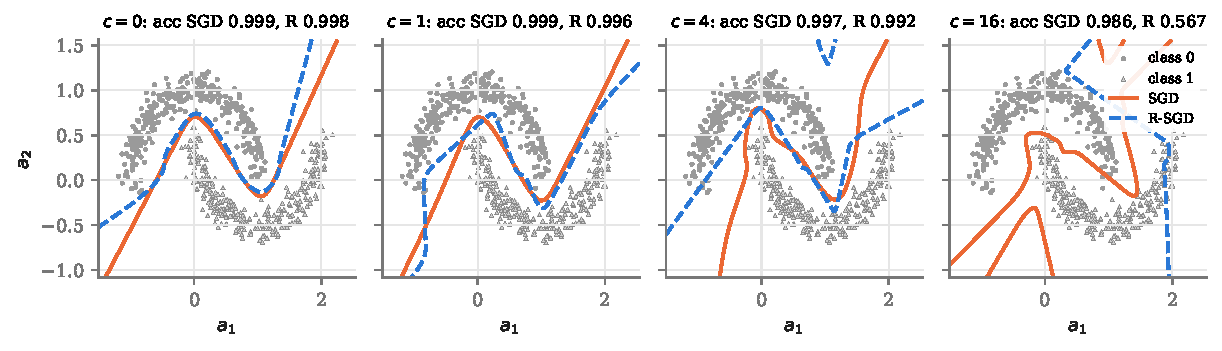
\includegraphics[width=\linewidth]{../fig3/mlp_boundaries.pdf}
\caption{Двухслойная сеть, сид оценки A-0: границы решения итоговых точек SGD и R-SGD в
исходных координатах и 600 тестовых точек. Вдали от данных границы экстраполируют по-разному,
даже когда обе разделяют полуокружности (две левые панели).}
\label{fig:mlp_bound}
\end{figure}

\subsection{Совпадают ли ранжирования по оптимизации и по предсказанию?}\label{sec:ranking}

\begin{itemize}
\item \textbf{Потери на обучении и на тесте: в основном да.} На фиксированном наборе данных
(схема B) знак $\Delta$ потерь на обучении предсказывал знак $\Delta$ потерь на тесте в 7--10 из
10 сидов во всех случаях, кроме сети при $c=1$ (3/10). В схеме A исключения — сеть при $c=1$
(5/10) и логистическая регрессия при $c=0$ (2/10), где разности $0.002$ тонут в разбросе между
наборами данных. Оба набора данных простые, и при 400 обучающих точках модели далеки от
переобучения.
\item \textbf{Потери на обучении и точность: при малом шуме нет.} Логистическая регрессия при
$c\le1$: совпадение 3--5/10; сеть при $c=0$: 3/10, хотя потери R-SGD на обучении в 5.8 раза
меньше. Меньшая кросс-энтропия здесь в основном означает более уверенные логиты на уже
правильно классифицированных точках. Логистическая регрессия находится на байесовской
точности, поэтому никакой оптимизатор не может её повысить; в сети оба метода на уровне $99.8\%$.
\item \textbf{При большом шуме все ранжирования совпадают} (7--10/10): шум портит саму границу, и
метод с меньшими потерями и классифицирует лучше.
\item Для обоих экспериментов вместе: меньшие потери на обучении, меньшие потери на тесте и
более высокая точность — разные результаты, как и сказано в критерии успеха задания. В этих
экспериментах R-SGD иногда добивался первых двух; более высокой точности, чем у SGD с той же
средней длиной шага, он не добился ни разу.
\end{itemize}

\section{Честная настройка и оценка}\label{sec:protocol}

\subsection{Сравнимые бюджеты}
Оба метода используют один размер батча $b=16$ (выбор с возвращением), одно число обновлений
($K=500$ для логистической регрессии, $K=3000$ для сети) и одно расписание
$\alpha_k=\alpha_0/\sqrt{1+k/50}$. Поэтому каждый запуск тратит ровно $bK$ вычислений градиента
примера: $8000$ и $48\,000$ соответственно, одинаково для SGD и R-SGD. Время замеряется только на
$K$ обновлениях, без контрольных точек оценки, и приводится в таблицах результатов
раздела~\ref{sec:sims}. В Python обновление R-SGD обходится в 2.6--4.4 раза дороже из-за
постоянных накладных расходов решателя. Сравниваются только обычный SGD и R-SGD.

\subsection{Выбор гиперпараметров}\label{sec:tuning}
\textbf{Протокол настройки.}
\begin{itemize}
\item Сетки: $\alpha_0\in\{0.1,0.3,1,3,10,30\}$ для обоих методов; $r\in\{0,0.25,0.5,0.75,1,1.25\}$
для R-SGD. $r=0$ включено, и R-SGD с $r=0$ — это SGD.
\item Данные для настройки: 3 сида настройки со своими наборами данных, инициализациями, батчами и
шумом, не пересекающиеся с сидами оценки; уровень шума при настройке $c=1$. Тестовые данные не
используются.
\item Критерий: среднее по сидам настройки значение потерь на валидации, усреднённых по последним
5 из 61 контрольной точки. Запуск считается неудачным, если потери на обучении становятся
бесконечными или превышают начальные в 50 раз.
\item Бюджеты поиска: SGD $6\times3=18$ запусков, R-SGD $36\times3=108$ запусков. Больший бюджет
даёт R-SGD преимущество (это минимум по большему числу шумных оценок); это обсуждается ниже.
\item После настройки параметры фиксируются и без изменений используются на всех уровнях шума.
\end{itemize}

\paragraph{Логистическая регрессия.}
\begin{figure}[H]
\centering
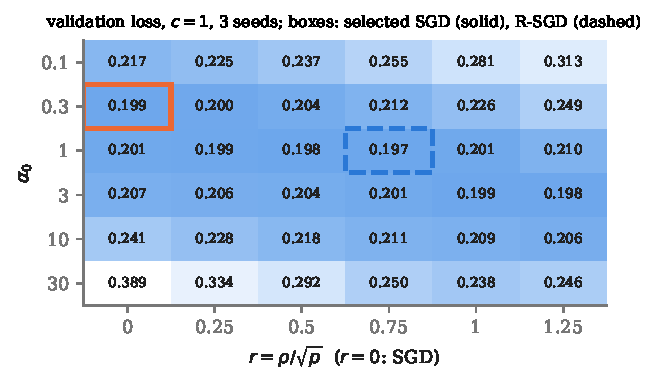
\includegraphics[width=0.49\linewidth]{../fig3/logreg_tuning.pdf}\hfill
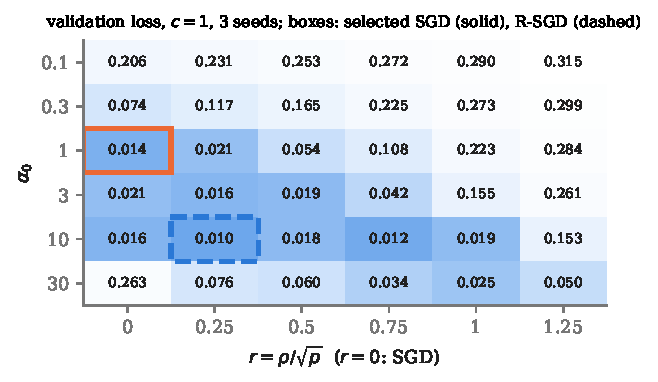
\includegraphics[width=0.49\linewidth]{../fig3/mlp_tuning.pdf}
\caption{Критерий настройки (средние потери на валидации, $c=1$, 3 сида настройки) для
логистической регрессии (слева) и сети (справа). Столбец $r=0$ — SGD. Рамки отмечают
выбранные настройки. (Подписи на рисунках на английском.)}
\label{fig:tuning}
\end{figure}

Выбрано: SGD $\alpha_0=0.3$; R-SGD $\alpha_0=1$, $r=0.75$ ($\rho=1.30$). Ни одна настройка не
лежит на краю сетки. Критерий очень плоский: 10 из 36 клеток отличаются от лучшей ($0.197$) не
более чем на $0.005$. Область малых значений идёт по диагонали: больший $\alpha_0$ компенсируется
большим $r$, например $(1,0.75)$, $(3,1)$, $(3,1.25)$ почти равны. Это и есть взаимодействие шага
обучения и радиуса, о котором спрашивает раздел 5(b): оба управляют эффективной длиной шага.

\paragraph{Сеть.}
Выбрано (рис.~\ref{fig:tuning}, справа): SGD $\alpha_0=1$; R-SGD $\alpha_0=10$, $r=0.25$
($\rho=1.44$). Ни одна настройка не на краю. Критерий R-SGD ($0.0104$) меньше, чем у SGD
($0.0138$), но поверхность нерегулярна: $(10,0)$, то есть SGD с $\alpha_0=10$, даёт $0.0156$,
$(10,0.5)$ — $0.0184$, $(10,0.75)$ — $0.0117$. Такие немонотонные соседи показывают, что разности
этого масштаба лежат в пределах шума оценки по 3 сидам. Последствия видны в разделе~\ref{sec:sim2}.

\subsection{Воспроизводимость и разброс}\label{sec:variability}
\textbf{Схемы оценки.} Две схемы по 10 сидов, парные по методам (одни и те же данные,
инициализация, индексы батчей и реализации шума $z_{k,i}$):
\begin{itemize}
\item \textbf{A} (меняется набор данных): каждый сид генерирует новые обучающую, валидационную и
тестовую выборки, новую инициализацию, новые батчи и новый шум. Разброс в A объединяет
неопределённость по наборам данных и случайность обучения.
\item \textbf{B} (только случайность обучения): набор данных A-сида 0 зафиксирован; меняются
инициализация, батчи и шум.
\end{itemize}
Погрешности: «среднее $\pm$ sd» — среднее и выборочное стандартное отклонение по 10 сидам
(разброс результатов). Для парных разностей «среднее $\pm$ h» даёт полуширину $h$
95\%-го $t$-интервала для средней разности, «победы» — число сидов, где R-SGD лучше (ничьи в
скобках).

\paragraph{Логистическая регрессия.}
\begin{center}
\small
\begin{tabular}{@{}ccccccccc@{}}
\toprule
& \multicolumn{4}{c}{sd потерь на тесте} & \multicolumn{4}{c}{sd точности на тесте} \\
\cmidrule(lr){2-5}\cmidrule(lr){6-9}
$c$ & SGD A & SGD B & R-SGD A & R-SGD B & SGD A & SGD B & R-SGD A & R-SGD B \\
\midrule
\tabinput{../tabs3/tab_lr_var.tex}
\bottomrule
\end{tabular}

\smallskip
Логистическая регрессия: разброс по наборам данных и случайности обучения (A) против разброса
только по случайности обучения (B).
\end{center}
При $c\le1$ доминирует разброс по наборам данных (sd в A в 2--7 раз больше, чем в B); при $c\ge4$
главным источником становится случайность обучения из-за добавленного шума.

\paragraph{Сеть.}
\begin{center}
\small
\begin{tabular}{@{}ccccccccc@{}}
\toprule
& \multicolumn{4}{c}{sd потерь на тесте} & \multicolumn{4}{c}{sd точности на тесте} \\
\cmidrule(lr){2-5}\cmidrule(lr){6-9}
$c$ & SGD A & SGD B & R-SGD A & R-SGD B & SGD A & SGD B & R-SGD A & R-SGD B \\
\midrule
\tabinput{../tabs3/tab_mlp_var.tex}
\bottomrule
\end{tabular}

\smallskip
Двухслойная сеть: разброс по наборам данных и случайности обучения (A) против разброса только
по случайности обучения (B).
\end{center}
Для сети разброс в B (случайность обучения, включая инициализацию) сравним с разбросом в A, в
отличие от логистической регрессии: невыпуклая модель чувствительна к инициализации и к
траектории. При 10 сидах сама оценка sd неопределённа примерно на $\pm25\%$, поэтому значимы
только большие отношения.

Ни один запуск не попал под критерий неудачи (потери на обучении бесконечны или превышают
начальные в 50 раз) ни в настройке, ни в оценке, ни в переборе. 8 запусков сети при $c=16$ с
итоговыми потерями выше начальных $\log2$ описаны в разделе~\ref{sec:sim2}.

\subsection{Чувствительность и длина шага}\label{sec:sens}
\textbf{Исследование чувствительности и контроль.} (i) Перебор радиуса $r\in\{0,\dots,2\}$ при настроенном
$\alpha_0$ для SGD, 5 сидов. (ii) Контроль длины шага: SGD с
$\alpha_0'=\alpha_0\cdot\overline{\|d_k\|/(\alpha_k\|g_k\|)}$, средним отношением шагов
соответствующих запусков R-SGD (нулевые шаги дают 0). Он запускается для зафиксированной
настройки и для каждой точки перебора на тех же сидах.

\paragraph{Логистическая регрессия.}
\begin{center}
\small
\setlength{\tabcolsep}{4pt}
\begin{tabular}{@{}cccccccc@{}}
\toprule
$c$ & \shortstack{отн.\\шага} & $\alpha_0'$ & потери R-SGD & \shortstack{потери SGD\\с той же длиной} & $\Delta$ (R $-$ контр.) & побед & \shortstack{точн.\\R / контр.} \\
\midrule
\tabinput{../tabs3/tab_lr_matched.tex}
\bottomrule
\end{tabular}

\smallskip
Зафиксированный R-SGD против SGD с той же средней длиной шага, схема A, 10 сидов (потери на
тесте).
\end{center}

При $c=0$ подобранный шаг в точности равен настроенному для SGD значению $0.3$, и методы равны
(5/10). При $c=1$ R-SGD выигрывает у контроля в 9/10 сидов на $0.003$ по потерям на тесте. При
$c\ge4$ контрольный SGD лучше, при $c=16$ — на $0.14$.

\begin{figure}[H]
\centering
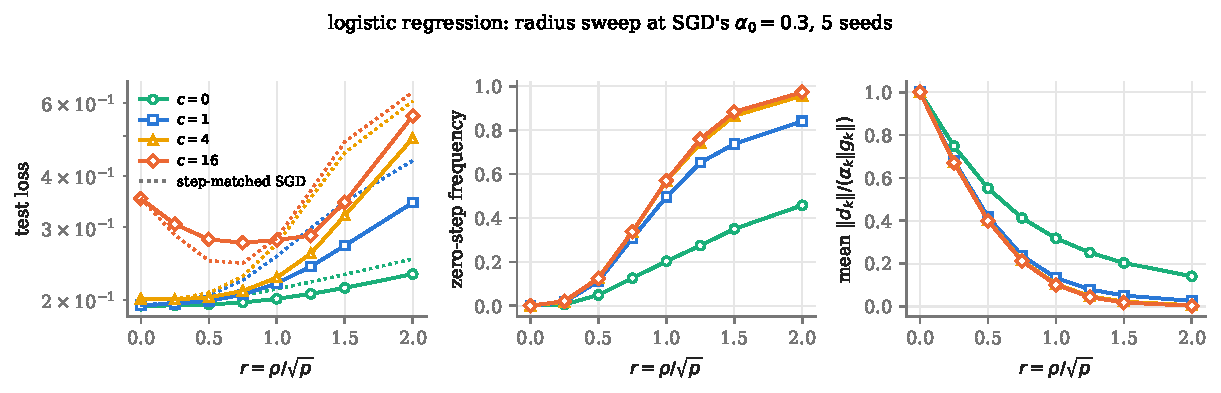
\includegraphics[width=\linewidth]{../fig3/logreg_sensitivity.pdf}
\caption{Логистическая регрессия, перебор радиуса при $\alpha_0=0.3$ (настройка SGD), 5 сидов.
Слева: потери на тесте R-SGD (сплошные) и SGD с той же длиной шага (пунктир). В центре: доля
нулевых шагов. Справа: среднее отношение $\|d_k\|/(\alpha_k\|g_k\|)$.}
\label{fig:lr_sens}
\end{figure}

\begin{center}
\small
\setlength{\tabcolsep}{4pt}
\begin{tabular}{@{}ccccccccc@{}}
\toprule
$c$ & $r$ & \shortstack{нулевые\\шаги} & \shortstack{отн.\\шага} & \shortstack{потери\\обуч.} & \shortstack{потери\\тест} & \shortstack{контр.\ SGD\\тест} & \shortstack{побед\\R} & точность \\
\midrule
\tabinput{../tabs3/tab_lr_sens.tex}
\bottomrule
\end{tabular}

\smallskip
Логистическая регрессия, перебор радиуса при $\alpha_0=0.3$ (средние по 5 сидам); $r=0$ — SGD.
\end{center}

\begin{itemize}
\item При $c\le4$ рост $r$ не снижает потери (не более чем на $0.0007$ при $r=0.25$, затем они
растут): при настроенном шаге SGD выигрывать нечего. Но R-SGD лучше SGD с той же средней длиной
шага при каждом $r$ в 5/5 сидов (один раз 4/5). Его сжатие мало в начале (большие градиенты,
высокое отношение сигнал/шум) и велико в конце, то есть работает как адаптивное уменьшение шага;
постоянное уменьшение теряет скорость в начале.
\item При $c=16$ значения $r=0.5$--$0.75$ снижают потери на тесте с $0.352$ до $0.275$, но
контрольный SGD даёт лучше ($0.246$, R-SGD выигрывает в 1/5): выигрыш — эффект длины шага.
\item Точность почти не меняется с $r$ (в пределах $0.002$ при $c\le4$), пока не начинают
доминировать нулевые шаги.
\end{itemize}

\paragraph{Сеть.}
\begin{center}
\small
\setlength{\tabcolsep}{4pt}
\begin{tabular}{@{}cccccccc@{}}
\toprule
$c$ & \shortstack{отн.\\шага} & $\alpha_0'$ & потери R-SGD & \shortstack{потери SGD\\с той же длиной} & $\Delta$ (R $-$ контр.) & побед & \shortstack{точн.\\R / контр.} \\
\midrule
\tabinput{../tabs3/tab_mlp_matched.tex}
\bottomrule
\end{tabular}

\smallskip
Двухслойная сеть: зафиксированный R-SGD против SGD с той же средней длиной шага, схема A,
10 сидов.
\end{center}

\begin{figure}[H]
\centering
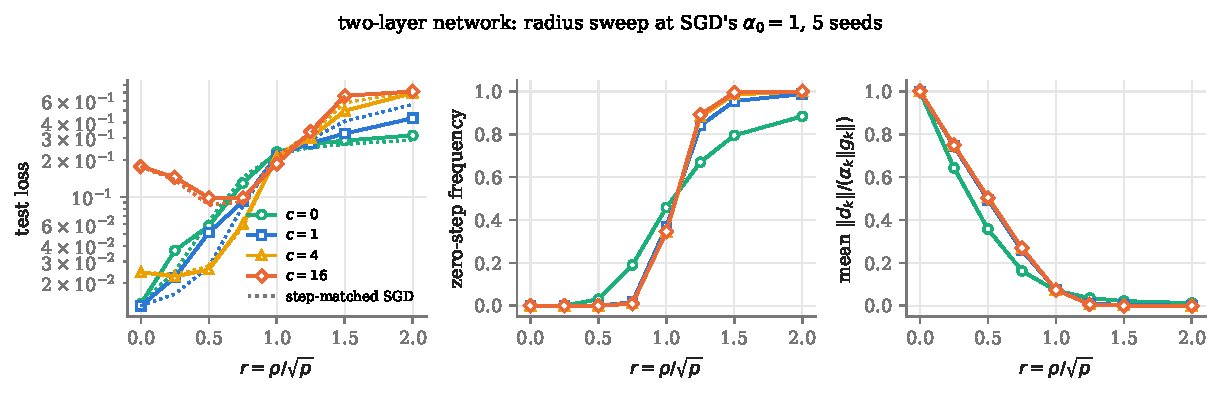
\includegraphics[width=\linewidth]{../fig3/mlp_sensitivity.pdf}
\caption{Двухслойная сеть, перебор радиуса при $\alpha_0=1$ (настройка SGD), 5 сидов. Слева:
потери на тесте R-SGD (сплошные) и SGD с той же длиной шага (пунктир). В центре: доля нулевых
шагов. Справа: среднее отношение шагов.}
\label{fig:mlp_sens}
\end{figure}

\begin{center}
\small
\setlength{\tabcolsep}{4pt}
\begin{tabular}{@{}ccccccccc@{}}
\toprule
$c$ & $r$ & \shortstack{нулевые\\шаги} & \shortstack{отн.\\шага} & \shortstack{потери\\обуч.} & \shortstack{потери\\тест} & \shortstack{контр.\ SGD\\тест} & \shortstack{побед\\R} & точность \\
\midrule
\tabinput{../tabs3/tab_mlp_sens.tex}
\bottomrule
\end{tabular}

\smallskip
Двухслойная сеть, перебор радиуса при $\alpha_0=1$ (средние по 5 сидам); $r=0$ — SGD.
\end{center}

\begin{itemize}
\item При $c\le1$ любое $r>0$ ухудшает результат; при $c=4$ эффект $r\le0.5$ в пределах шума.
\item При $c=16$ значения $r=0.5$--$0.75$ улучшают потери на тесте с $0.176$ до $0.098$ и
точность с $0.953$ до $0.968$, но контрольный SGD ещё лучше ($0.086$; R-SGD выигрывает 2/5 и
1/5). В режиме доминирующего шума робастный шаг ведёт себя как укороченный шаг SGD.
\item \textbf{Нулевые шаги до минимума.} При $r\ge1$ доля нулевых шагов скачком растёт до
35--100\%, и обучение останавливается при точности $0.91$--$0.50$. При $c=4,16$ и $r=2$ сеть
практически не движется (99.9--100\% нулевых шагов, точность $0.50$). Объяснение (раздел~\ref{sec:critical}(b)): когда
доминирует шум, $g_k^TS_k^{-1}g_k$ близко к своему значению в стационарной точке независимо от
$\theta_k$, поэтому проверка нулевого шага не может определить, близка ли итерация к минимуму.
\end{itemize}

\paragraph{Вывод исследования чувствительности.} Рост радиуса в основном укорачивает шаг. Везде,
где R-SGD улучшал результат SGD при переборе, SGD с той же средней длиной шага давал то же или
лучше, кроме логистической регрессии при $c\le4$. Там сжатие R-SGD, зависящее от отношения
сигнал/шум, выигрывало у постоянного уменьшения шага, но только по потерям. Радиусы
$\rho\gtrsim\sqrt p$ порождают нулевые шаги далеко от любого минимума (раздел~\ref{sec:critical}).


\section{Критический анализ}\label{sec:critical}

В ответах ниже разделены три вида утверждений: математические результаты (раздел~1), механизмы,
выведенные при явно указанных предположениях, и эмпирические факты для двух наших задач и
настроек.

\subsection{(a) Когда R-SGD помогает?}

\textbf{Свидетельства в пользу.}
\begin{itemize}
\item \emph{Малый шум, логистическая регрессия.} R-SGD немного, но устойчиво снижал потери. При
$c=1$ его потери на тесте были на $0.0027$ ниже, чем у SGD с той же средней длиной шага, в 9/10
сидов. При переборе радиуса при $c\le4$ он выигрывал у такого SGD при каждом радиусе в 5/5 сидов
(один раз 4/5). Здесь дисперсии координат различаются и меняются во времени, поэтому сжатие
работает как адаптивное, зависящее от отношения сигнал/шум уменьшение шага. Оно слабое в начале,
когда градиенты велики и надёжны, и сильное вблизи минимума. Постоянное уменьшение шага с тем же
средним этого не воспроизводит.
\item \emph{Страховка для больших шагов при малом шуме.} Настройка выбрала для R-SGD бо́льшие шаги
($3\times$ и $10\times$ шага SGD), которые его сжатие сделало применимыми при $c\le1$. В сети при
$c=0$ это дало в $5.8$ раза меньшие потери на обучении, чем у настроенного SGD.
\end{itemize}

\textbf{Свидетельства против.}
\begin{itemize}
\item Выигрыш сети — выигрыш длины шага. SGD со средней длиной шага R-SGD достиг тех же потерь на
обучении ($0.0018$ против $0.0019$) и меньших потерь на тесте ($0.0065$ против $0.0082$).
\item Выигрыша в точности нет нигде: логистическая регрессия на байесовском уровне, сеть на
уровне $99.8\%$.
\item При шуме зафиксированные настройки R-SGD были хуже SGD в обоих экспериментах, а при
переборе каждое улучшение R-SGD при $c=16$ воспроизводилось или превосходилось SGD с той же
длиной шага.
\end{itemize}

\textbf{Механизм (выведен, затем подтверждён).} Когда добавленный шум доминирует, все
$\widehat s_{k,j}\approx\sigma^2/b$, так что $S_k\approx sI$, и работает пункт 1(d). Поскольку $g_k$ в
основном шум, $\norm{g_k}^2\approx ps$, и при $\rho=r\sqrt p$
\begin{equation*}
\frac{\norm{d_k}}{\alpha_k\norm{g_k}}\approx1-\frac{\rho\sqrt s}{\sqrt{ps}}=1-r .
\end{equation*}
Измерено для сети при $c\ge4$: $0.748,\ 0.505,\ 0.269$ при $r=0.25,0.5,0.75$. При $p=3$ согласие
грубее ($0.67, 0.40, 0.21$), потому что в трёх измерениях $\norm{g_k}$ флуктуирует сильнее. В этом
режиме R-SGD в первом приближении — это SGD с более коротким шагом и тем же направлением, поэтому он
не должен превосходить SGD, шаг которого настроен при том же уровне шума. Во втором приближении он
хуже постоянного уменьшения: множитель $1-\rho\sqrt s/\norm{g_k}$ растёт с $\norm{g_k}$, и самые
большие, самые шумные градиенты сжимаются меньше всего. Робастный шаг выполняет мягкое пороговое
отсечение нормы градиента, а не уменьшение дисперсии.

\textbf{Ответ.} В наших экспериментах R-SGD помогал только при трёх условиях: (i) неопределённость
анизотропна и меняется во времени, так что его сжатие отличается от постоянного уменьшения шага;
(ii) оценка $S_k$ надёжна ($b\ge8$); (iii) мерой служат потери, а не точность. При доминирующем
изотропном шуме он сводится к укороченному шагу SGD и не может превзойти настроенный SGD.

\subsection{(b) Взаимодействие радиуса, ковариации и шага обучения}

\begin{itemize}
\item \textbf{Радиус и шаг обучения вместе задают длину шага.} Для ненулевого шага
$d_{k,j}=-\alpha_k\,\tau g_{k,j}/(\tau+\alpha_k\rho s_{k,j})$ зависит от произведения
$\alpha_k\rho s_{k,j}$. Поверхности настройки показывают этот компромисс: в логистической регрессии
почти оптимальные клетки лежат на диагонали, и $(\alpha_0,r)=(1,0.75)$, $(3,1)$, $(3,1.25)$ почти
равны (рис.~\ref{fig:tuning}). Больший шаг обучения компенсируется бо́льшим радиусом.
\item \textbf{Решение о нулевом шаге не зависит от $\alpha_k$} (раздел~1(c)). Оно зависит только от
$\rho$ и $S_k$. Таким образом, $\alpha$ масштабирует ненулевые шаги, а $\rho$ один решает, где метод
перестаёт двигаться.
\item \textbf{Ковариация зависит от батча и шума.} $S_k\approx\Sigma/b$, где $\Sigma$ включает
дисперсию выбора примеров и $\sigma^2I$. Поэтому радиус неопределённости в единицах градиента,
$\rho\sqrt{s_{k,j}}$, при шуме ведёт себя как $\rho\sigma/\sqrt b$. Робастная поправка убывает как
$1/\sqrt b$: с $0.237$ до $0.117$ между $b=64$ и $b=256$ (раздел~2). Одно и то же $\rho$ означает
разную робастность при разных размерах батча и уровнях шума, поэтому $\rho$ нужно настраивать при
используемом $b$. Масштаб $\rho=r\sqrt p$ делает его сравнимым между моделями.
\item \textbf{Нулевые шаги до достижения минимума.} При точной $S=\Sigma/b$ нулевые шаги возникают
примерно там, где $b\,\nabla f^T\Sigma^{-1}\nabla f\le\rho^2$. Эта область окружает минимум, но
далеко простирается вдоль направлений малой кривизны и большого шума. В зашумлённой квадратичной
задаче ($\sigma=4$, $b=8$, $\rho=2.45$) её полуоси равны $6.9$ и $0.43$, и нулевые шаги случались
при $f$ до $2.94$ ($f(\theta_0)=10$). При сильном добавленном шуме
$g_k^TS_k^{-1}g_k\approx\sum_jt_j^2$, где $t_j$ имеют распределение Стьюдента с $b-1$ степенями
свободы \emph{в любой} точке $\theta$. Тогда нулевые шаги почти неизбежны при
$r>\sqrt{(b-1)/(b-3)}=1.07$. Сеть останавливалась на точности $0.50$--$0.92$ при $r\ge1$, а при
$r=2$, $c\ge4$ вообще не покидала начальной точки. Даже без шума добавка $\varepsilon_k$ создаёт
область нулевого шага: при $S_k=\varepsilon I$ квадратичная задача сошлась к $f=\rho^2\varepsilon/2$,
что измерено с точностью до девяти знаков.
\end{itemize}

\subsection{(c) Следует ли из меньших потерь на обучении более высокая точность?}

Нет, не в наших экспериментах.
\begin{itemize}
\item \textbf{Сеть, $c=0$.} Потери R-SGD на обучении в $5.8$ раза меньше (10/10 сидов), потери на
тесте меньше в 9/10 сидов. Но точность не выше: $0.9977$ против $0.9982$, 3 победы и 2 ничьи. Знак
разности потерь на обучении предсказал разность точностей лишь в 3/10 сидов.
\item \textbf{Логистическая регрессия.} Оба метода достигают байесовской точности ($0.922$ против
$0.923$), поэтому никакой оптимизатор не может её повысить. Разности потерь $0.002$--$0.003$
сдвигают линейную границу пренебрежимо мало; совпадение ранжирования с точностью 3--5/10.
\item \textbf{Объяснение.} Кросс-энтропия продолжает убывать, когда логиты на правильно
классифицированных точках становятся увереннее, а точность учитывает только знак. Когда оба метода
правильно классифицируют почти все точки, меньшие потери означают бо́льшие отступы, а не меньше ошибок.
\item \textbf{Потери на обучении и на тесте} согласовывались чаще: в 7--10/10 сидов на фиксированном
наборе данных, так как 400 обучающих точек для таких малых моделей далеки от режима переобучения.
\item \textbf{При большом шуме} все три ранжирования совпадали (7--10/10, SGD лучше), потому что шум
портит саму границу решения.
\end{itemize}

\subsection{(d) Ограничения и сфокусированный следующий эксперимент}

\textbf{Ограничения.}
\begin{itemize}
\item \textbf{Настройка.} Три сида настройки на одном уровне шума и бо́льшая сетка для R-SGD (108
против 18 запусков). Это дало видимое «проклятие победителя»: выбор R-SGD для сети предсказывал
выигрыш при $c=1$, но при оценке при $c=1$ проиграл (потери на валидации $0.0230$ против $0.0114$).
Фиксация настроек при $c=1$, требуемая протоколом, определяет исход при $c\ge4$.
\item \textbf{Модель шума.} Добавленный шум гауссовский, изотропный и несмещённый. По механизму из
пункта (a) это в точности случай, когда R-SGD сводится к укороченному шагу SGD. Анизотропный, с
тяжёлыми хвостами или смещённый шум не проверялся.
\item \textbf{Диагональная $S_k$} игнорирует корреляции между 33 параметрами сети.
\item \textbf{Масштаб.} Двумерные данные, 400 обучающих точек и замеры времени в чистом Python, где
постоянные накладные расходы решателя делают обновление R-SGD в 2.6--4.4 раза медленнее.
\end{itemize}

\textbf{Сфокусированный следующий эксперимент: анизотропный шум и настройка с равным бюджетом на
каждом уровне шума.}
\begin{itemize}
\item \emph{Постановка.} Добавлять шум только в один блок параметров, например в 16 весов первого
слоя сети, при $c\in\{4,16\}$; остальные 17 координат остаются чистыми.
\item \emph{Настройка.} Настраивать SGD и R-SGD отдельно на каждом $c$ с равными бюджетами поиска
(по 36 настроек, с более частой сеткой $\alpha_0$ для SGD) и 10 сидами настройки.
\item \emph{Оценка.} Сравнивать на 10 парных сидах с настроенным SGD и с SGD той же длины шага.
\item \emph{Почему это проверяет нужное.} При анизотропном шуме $S_k$ далека от $sI$, и
покоординатное сжатие нельзя имитировать никаким скалярным шагом.
\item \emph{Правило решения.} R-SGD имеет настоящее преимущество робастности, если его потери на
тесте ниже, чем у обоих контролей, и 95\%-й парный интервал не содержит нуля; иначе наш вывод
остаётся в силе.
\end{itemize}


\section{Воспроизводимость и пакет кода}\label{sec:repro}

\textbf{Структура пакета} (папка \texttt{Mini-project SGD vs R-SGD}).
\begin{center}
\small
\begin{tabular}{@{}p{0.33\linewidth}p{0.6\linewidth}@{}}
\toprule
Путь & Содержимое \\
\midrule
\texttt{Report/} & этот отчёт (EN и RU, PDF) и прежние отчёты по разделам \\
\texttt{Report/source/} & исходники LaTeX с папками \texttt{../fig/}, \texttt{../fig3/}, \texttt{../tabs3/} \\
\texttt{Code/rsgd.py} & оценка (4), решатель для (2), цикл SGD/R-SGD, оракулы градиента, генераторы данных, проверка конечными разностями \\
\texttt{Code/checks\_section2.py} & все проверки и рисунки раздела~\ref{sec:impl} \\
\texttt{Code/sim3\_core.py} & разбиение данных, стандартизация по обучающей выборке, цикл обучения с чистой оценкой и замером времени \\
\texttt{Code/sim\_section3.py} & настройка, оценка (схемы A, B), перебор радиуса, контроль длины шага, рисунки \\
\texttt{Code/make\_tables3.py} & таблицы LaTeX разделов~\ref{sec:sims}--\ref{sec:protocol} \\
\texttt{Results/} & \texttt{results\_section2.json}, \texttt{results\_section3.json}, \texttt{tables\_section3.json}, \texttt{curves\_section3.npz} \\
\texttt{Presentation/} & слайды (PDF) и подготовленные ответы на вероятные вопросы \\
\bottomrule
\end{tabular}
\end{center}

\textbf{Команды} (одно ядро процессора):
\begin{lstlisting}
cd Code
python checks_section2.py      # Section 2, about 20 s: results_section2.json, fig/
python sim_section3.py run     # Sections 3-4, about 3 min: results_section3.json,
                               #   curves_section3.npz, fig3/
python make_tables3.py         # LaTeX tables used in Sections 3-4
\end{lstlisting}
Отчёты пересобираются двукратным запуском \texttt{xelatex} в \texttt{Report/source/}.

\textbf{Случайность.}
\begin{itemize}
\item Раздел~\ref{sec:impl}: главный сид $20261117$, восемь независимых дочерних потоков
из\\ \texttt{SeedSequence(20261117).spawn(8)}.
\item Разделы~\ref{sec:sims}--\ref{sec:protocol}: главный сид $20261118$. У каждого сида четыре
независимых потока (данные, инициализация, индексы батчей, шум градиента) из
\texttt{SeedSequence([20261118, sim, kind, seed])}:
  \begin{itemize}
  \item \texttt{sim}: 1 для логистической регрессии, 2 для сети;
  \item \texttt{kind}: 0 для сидов настройки 0--2, 1 для сидов схемы A 0--9, 2 для сидов схемы B
  0--9 (их поток данных — поток A-сида 0).
  \end{itemize}
\item Границы решения показаны для A-сида 0. SGD и R-SGD используют для каждого сида одинаковые
потоки (общие случайные числа).
\end{itemize}

\textbf{Искажение и оценка.} Шум добавляется только к наблюдаемым градиентам примеров $v_{k,i}$.
Целевая функция, данные, потери и точности всегда вычисляются на чистых данных, а тестовые данные
никогда не используются при настройке.

\textbf{ПО.} Python 3.13, NumPy 2.5.3, SciPy 1.18.1, Matplotlib 3.11.2, везде float64.
CVXPY 1.9.3 (Clarabel) используется только для одной перекрёстной проверки.


\begin{thebibliography}{9}
\bibitem{bental} A.~Ben-Tal, L.~El Ghaoui, A.~Nemirovski. \emph{Robust Optimization}. Princeton
University Press, 2009.
\bibitem{bottou} L.~Bottou, F.~E.~Curtis, J.~Nocedal. Optimization methods for large-scale machine
learning. \emph{SIAM Review} 60(2):223--311, 2018.
\bibitem{boyd} S.~Boyd, L.~Vandenberghe. \emph{Convex Optimization}. Cambridge University Press,
2004.
\bibitem{byrd} R.~H.~Byrd, G.~M.~Chin, J.~Nocedal, Y.~Wu. Sample size selection in optimization
methods for machine learning. \emph{Mathematical Programming} 134:127--155, 2012.
\bibitem{more} J.~J.~Moré, D.~C.~Sorensen. Computing a trust region step. \emph{SIAM J.\ Sci.\
Stat.\ Comput.} 4(3):553--572, 1983.
\bibitem{nesterov} Yu.~Nesterov. \emph{Introductory Lectures on Convex Optimization}. Kluwer, 2004.
\bibitem{nocedal} J.~Nocedal, S.~J.~Wright. \emph{Numerical Optimization}, 2nd ed. Springer, 2006.
\bibitem{robbins} H.~Robbins, S.~Monro. A stochastic approximation method. \emph{Annals of
Mathematical Statistics} 22(3):400--407, 1951.
\bibitem{phan} A.-H.~Phan. Homework mini-project: SGD versus Robust SGD under gradient uncertainty.
Course assignment, 2026.
\end{thebibliography}

\appendix
\section{Решатель}\label{app:solver}
\begin{lstlisting}[language=Python]
def robust_step(g, s, alpha, rho, tol=1e-14, maxit=100):
    kappa2 = np.sum(g * g / s)                    # g^T S^{-1} g
    if rho == 0.0:                                # SGD
        return -alpha * g
    if kappa2 <= rho * rho:                       # zero-step rule (3)
        return np.zeros_like(g)
    a = alpha**2 * s * g * g                      # q(tau) = sum a/(tau+c)^2
    c = alpha * rho * s
    def psi_and_deriv(tau):
        den = tau + c
        q, dq = np.sum(a / den**2), -2.0 * np.sum(a / den**3)
        return q**-0.5 - 1.0, -0.5 * q**-1.5 * dq
    lo, hi = 0.0, alpha * np.sqrt(np.sum(s * g * g))   # bracket
    tau = 0.0
    psi, dpsi = psi_and_deriv(tau)
    for it in range(maxit):
        tau_new = tau - psi / dpsi                # Newton (monotone from 0)
        if not (lo < tau_new <= hi):
            tau_new = 0.5 * (lo + hi)             # safeguard, never used
        step, tau = abs(tau_new - tau), tau_new
        psi, dpsi = psi_and_deriv(tau)
        lo, hi = (tau, hi) if psi < 0 else (lo, tau)
        if abs(psi) <= tol or step <= 1e-15 * tau:
            break
    return -alpha * tau * g / (tau + c)
\end{lstlisting}

\section{Где находится каждый требуемый результат}\label{app:map}
\begin{center}
\small
\begin{tabular}{@{}p{0.5\linewidth}p{0.42\linewidth}@{}}
\toprule
Требование задания & Где \\
\midrule
1(a)--(e) вывод, оптимальность, условное убывание & раздел~\ref{sec:derivation} \\
Решатель, критерий остановки, стоимость & раздел~\ref{sec:solver} \\
2(a) реализация, наблюдения градиента & раздел~\ref{sec:oracles} \\
2(b) нулевой радиус, изотропная формула, нулевой шаг, проверка 1(d) & раздел~\ref{sec:checks} \\
2(c) размер батча & раздел~\ref{sec:batch} \\
2(d) воспроизводимость реализации & разделы~\ref{sec:repro2}, \ref{sec:repro} \\
3: кривые потерь при всех уровнях шума & рис.~\ref{fig:lr_curves}, \ref{fig:mlp_curves} \\
3: итоговые потери, точность, время, нулевые шаги & таблицы в разделах~\ref{sec:sim1}, \ref{sec:sim2} \\
3: границы решения для указанного сида & рис.~\ref{fig:lr_bound}, \ref{fig:mlp_bound} \\
3: ранжирование по оптимизации и предсказанию & раздел~\ref{sec:ranking} \\
4.1--4.4 бюджеты, настройка, разброс, чувствительность & раздел~\ref{sec:protocol} \\
5(a)--(d) критический анализ & раздел~\ref{sec:critical} \\
Участники, вклад, литература, код, результаты & титульная часть, список литературы, раздел~\ref{sec:repro} \\
\bottomrule
\end{tabular}
\end{center}


\end{document}
